\documentclass{article}
\usepackage{amsmath}
\usepackage{amssymb}
\usepackage{amsthm}
\usepackage{prooftree}
\usepackage{algorithm,algorithmic}
\usepackage{float}
\usepackage[svgnames]{xcolor}

\usepackage{tikz}
\usetikzlibrary{arrows,automata}

% Proof rules and SOS rules.
\newcommand{\proofrule}[3][]{#1 \frac{\raisebox{.7ex}{\normalsize{$#2$}}}
  {\raisebox{-1.0ex}{\normalsize{$#3$}}}}

  % Modal equation systems
\newcommand{\E}{\mathcal{E}}
\newcommand{\eqmu}{\stackrel{\mu}{=}}
\newcommand{\eqnu}{\stackrel{\nu}{=}}
\newcommand{\eqsigma}{\stackrel{\sigma}{=}}
\newcommand{\lhs}{\mathsf{lhs}}
\newcommand{\rhs}{\mathsf{rhs}}

\newcommand{\placeholder}[1][]{\pi_{#1}}

\newcommand{\loc}{l}
\newcommand{\region}{\mathit{cc}}

\newcommand{\suc}{\mathit{succ}}
\newcommand{\pre}{\mathit{pred}}
\newcommand{\inv}{\mathit{inv}}
\newcommand{\post}{\mathit{post}}
\newcommand{\wpre}{\mathit{wp}}

\newcommand{\var}[1]{\ensuremath{\mathit{#1}}}
\newcommand{\method}[1]{\ensuremath{\mathbf{#1}}}
\newcommand{\true}{\texttt{true}}
\newcommand{\false}{\texttt{false}}

\usepackage[textwidth=3.2cm]{todonotes}
%\setlength{\marginparwidth}{3.2cm}
\newcommand{\jk}[2][]{\todo[#1]{JK: #2}}

\title{Implementation notes for TimeSolver}
\author{Jeroen J.A. Keiren}

\begin{document}

\maketitle

In this note we describe the proof rules for $\mu$-calculus model checking of
timed automata as they are implemented in TimeSolver. We stick as close as
possible to the implementation. The rules were described originally
in~\cite{ZC:05forte,ZC:05rtss,Zhang:05}, and the rules with placeholder stem from~\cite{FC:14}. A
more elaborate discussion of (some of) the proof rules can be found
in~\cite{FC:14report}.

The proof rules are implemented in the file \texttt{proof.hh}. This is a
header-only implementation to allow the compiler to inline wherever possible.
The class \texttt{prover} supports proof rules without placeholder, named
\texttt{do\_proof\_*}, and proof rules with placeholder, named
\texttt{do\_proof\_place\_*}. Note that the rules without placeholders can call
the rules with placeholders, but not the other way around. The methods with
placeholder correspond to those proof rules in which a placeholder is present in
the goal. 

Below we describe each of the proof rules as they are implemented in the tool.

\section{Predicate variables}
The cases where the proof goal is a predicate variable is handled by the rules
\texttt{do\_proof\_predicate} and \texttt{do\_proof\_place\_predicate}.

\[
\proofrule
{(\loc, \region) \vdash X}
{(\loc, \region) \vdash \phi}
%
\quad
%
\proofrule
{(\loc, \region), \placeholder \vdash X}
{(\loc, \region), \placeholder \vdash \phi}
\]
Where $X \eqsigma \phi \in \E$ is an equation in the PES.

\subsection{Detecting cycles/finding companion nodes}
When we encounter a predicate variable, we need to decide whether the proof is successful or unsuccessful, or whether we need to actually apply the proof rule and continue on the right hand side. This hinges on deciding whether the proof branch ending in the current proof node $\mathbf{n}$ labelled with sequent $(\loc, \region) \vdash X$ is complete. In other words, we need to determine whether it has a \emph{companion node} in the proof tree. For this, we need to distinguish two cases:
\begin{itemize}
  \item If $X$ is a $\nu$-variable, then a proof node $\mathbf{m}$ on the path from the root of the proof tree to $\mathbf{n}$ is a companion node of $\mathbf{n}$ iff it is labelled with the sequent $(\loc', \region') \vdash X$, such that $\loc = \loc'$, and $\region \subseteq \region'$, and there is no node $\mathbf{m'}$ on the path from $\mathbf{m}$ to $\mathbf{n}$ such that $\mathbf{m'}$ is labelled with $(\loc'', \region'') \vdash Y$ for $\mu$-variable $Y$ defined before $X$ in $\mathcal{E}$.
  \item If $X$ is a $\mu$-variable, then a proof node $\mathbf{m}$ on the path from the root of the proof tree to $\mathbf{n}$ is a companion node of $\mathbf{n}$ iff it is labelled with the sequent $(\loc', \region') \vdash X$, such that $\loc = \loc'$, and $\region' \subseteq \region$, and there is no node $\mathbf{m'}$ on the path from $\mathbf{m}$ to $\mathbf{n}$ such that $\mathbf{m'}$ is labelled with $(\loc'', \region'') \vdash Y$ for $\nu$-variable $Y$ defined before $X$ in $\mathcal{E}$.
\end{itemize}
Note: in the alternation free case, there can never be a cancelling node $\mathbf{m'}$ on the path from $\mathbf{m}$ to $\mathbf{n}$, so we can omit the check for that.

Detecting companion nodes in the implementation is performed by maintaining two stacks, containing $\nu$-sequents and $\mu$-sequents, respectively. Every time the fixed point rule is applied, the goal-sequent is pushed onto the appropriate stack, and the subgoal is calculated recursively. When the recursive call completes, the sequent needs to be popped from the stack again since otherwise it might interfere with other subproofs.

The stacks need to support the following operations:
\begin{itemize}
  \item push a sequent $(\loc, \region) \vdash X$ onto the stack,
  \item pop a sequent from the stack,
  \item given a sequent $(\loc, \region) \vdash X$, determine whether the stack contains a sequent $(\loc, \region') \vdash X$, such that $\region \subseteq \region'$, in case $X$ is a $\nu$-variable, and $\region' \subseteq \region$, in case $x$ is a $\mu$-variable.
\end{itemize}
This results in the following code.

\begin{algorithm}[H]
  \caption{$\method{do\_proof\_predicate}(\loc, \region, \phi)$}
  \begin{algorithmic}
  \STATE \COMMENT{Assume $\phi = X$, and $X \stackrel{\mu/\nu}{=} \phi_X \in \mathcal{E}$}
  \STATE \COMMENT{There are 2 caches: $C_\mu$, $C_\nu$, that contain previously detected least- and greatest fixed point sequents, respectively.}
  
  \IF{Parity of $X$ is $\nu$}
    \IF{$\exists (X, \loc, \region') \in C_\nu . \region \subseteq \region'$}
      \RETURN $\mathit{true}$
    \ELSE
      \STATE $\method{push}((X, \loc, \region), C_\nu)$
      \STATE $\var{result} \gets \method{do\_proof}(\loc, \region, \phi_X)$
      \STATE $\method{pop}(C_\nu)$
    \ENDIF
  \ELSE[Parity of $X$ is $\mu$]
    \IF{$\exists (X, \loc, \region') \in C_\mu . \region' \subseteq \region$}
      \RETURN $\mathit{false}$
    \ELSE
      \STATE $\method{push}((X, \loc, \region), C_\mu)$
      \STATE $\var{result} \gets \method{do\_proof}(\loc, \region, \phi_X)$
      \STATE $\method{pop}(C_\mu)$
    \ENDIF
  \ENDIF
\end{algorithmic}
\end{algorithm}

\subsection{Optimizing the proof: caching known true/false sequents}
An orthogonal caching structure keeps track of sequents that have previously been determined to be true/false. Given the structure of the proofs, the caching here is also restricted to sequents of the form $(\loc, \region) \vdash X$. Intuitively, this allows the tool to save the work of computing the same subtree multiple times.

In the implementation, we maintain four caches:
\begin{itemize}
  \item $C_{pt}$ for possibly true sequents
  \item $C_{pf}$ for possibly false sequents
  \item $C_{t}$ for known true sequents
  \item $C_{f}$ for known false sequents
\end{itemize}
The possibly true/false caches contain those sequents for which we have detected a fixed-point cycle, but for which we have not yet completed the proof of the right hand side of the sequent. This is still helpful in saving work when multiple subproofs refer to the same fixed point variable.

The known true/false caches contain those sequents for which we have completed a proof of the right hand side.

Given a sequent $(\loc, \region) \vdash X$ we need to be able to determine the following:
\begin{itemize}
  \item Determine whether $C_{pt}$ or $C_{t}$ contains a sequent $(\loc, \region') \vdash X$ such that $\region \subseteq \region'$.
  \item Determine whether $C_{pf}$ of $C_{f}$ contains a sequent $(\loc, \region') \vdash X$ such that $\region' \subseteq \region$.
\end{itemize}
Intuition here is as follows: in case we find a true sequent in the cache, and every state in the sequent that we need to prove is part of that cached sequent, we have a successful proof (this is consistent with the Thinning rule in the proof system); in case we find a false sequent in the cache that is a subset of the sequent that we try to prove, likewise, we conclude that we found a false sequent. Why this is the case can be seen intuitively from an alternative reading of the sequents: $\lnot((\loc, \region') \implies X)$ and $(\loc, \region') \implies (\loc, \region)$ together imply $\lnot((\loc, \region) \implies X)$.

Note that, in some instances, in one branch of the proof we have concluded that a sequent is possibly true, and later observe that sequent to be false, or the other way around. An example of a case in which this happens is the following. Consider the timed automaton with a single state $s$, and the property $X \stackrel{\nu}{=} [-]X \land \mathit{false}$.

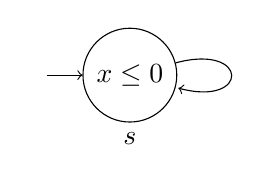
\begin{tikzpicture}
\node[state,initial left, initial text={}, label={below:$s$}] (s) {$x \leq 0$};
\draw (s) edge[loop right] (s);
\end{tikzpicture}

The proof here is unsuccessful, but when we look at the structure of the proof (shown below) we see that in the first branch of the proof, we detect a greatest fixed point cycle, and assume that the property holds.

\[
\proofrule
{(s,x \leq 0) \vdash X}
{
  \proofrule[\land]
  {(s,x \leq 0) \vdash [-]X \land \mathit{false}}
  {
    \proofrule[{[-]}]
    {(s,x \leq 0) \vdash [-]X}
    {
      (s,x \leq 0) \vdash X
    }
    \quad
    (s,x \leq 0) \vdash \mathit{false}
  }
}
\]
The second time we observe the sequent $(s, x \leq 0) \vdash X$, that exact sequent is in the greatest fixed point cache, and we conclude that the sequent is possibly true, and we store it in the known-true cache. However, once we consider the second branch, $(s, x \leq 0) \vdash \mathit{false}$, and propagate the result back, we conclude that $(s, x \leq 0) \vdash X$ (in the first sequent) is false, so we need to move the sequent from the possibly true cache to the false cache. Only then do we conclude that the proof is unsuccessful. Note that, when we would have observed the right hand side of the sequent is true, it would have been moved from the possibly true cache to the true cache.

In general, the caching mechanism works as follows.
\begin{itemize}
  \item When a sequent $(\loc, \region) \vdash X$ is observed, we check the following:
  \begin{itemize}
    \item is $(\loc, \region) \vdash X \in C_{t} \cup C_{pt}$ or $(\loc, \region) \vdash X \in C_{f} \cup C_{pf}$; in that case, we have found the solution for the current sequent.
    \item otherwise, proceed as in the case without caching to compute the solution the right hand side of $X$ in $\mathcal{E}$; in the case a cycle is detected, the result is added to the $C_{pt}$ when the parity of $X$ is $\nu$, and $C_{pf}$ otherwise.
    \item when the solution of the right hand side is computed, the sequent is removed from the $C_{pf}$ and $C_{pt}$ caches, and added to $C_f$ or $C_t$ depending on the obtained result.
  \end{itemize}
\end{itemize}
\todo{Argue why the possibly true and true cache can be combined in the implementation, although they are conceptually separate things; and likewise for the false cache}

\todo{The following is the reasoning behind not purging the caches in a backward way}
So, why don’t we have to purge anything from the caches?
This relies on the following observations.
\begin{itemize}
\item Remember that we maintain a stack of fixed point sequents that we have seen from the root of the proof tree until the current proof node.
\item Suppose we are in a proof node that is a sequent $(\loc,\region) \vdash X$; a value for this proof node is only cached if its a leaf
  \begin{itemize}
	  \item Since it is a leaf, it has a companion node, and
	  \item On the path from the companion node to the leaf, there is no sequent that refers to a predicate variable $Y$ for which $Y$ is of different parity, and it appears before $X$ in the MES.
    \item The sequent $(\loc,\region) \vdash X$ can, at this point be cached as possibly true/false; not as definitely true/false.
  \end{itemize}
\item The sequent $(\loc,\region) \vdash X$ is moved from possibly true/false to known true/false precisely when we have completed solving the entire subtree rooted at the companion node $(\loc,\region) \vdash X$.
\item Given the previous point, all nodes on the path from the root of the proof tree to the companion node are, when they are cached, in the possibly true/false cache, and not yet know to be true/false (if it would have been in the known true/false cache, we would not have continued down into the proof, but have used the cached value. This is interesting in the following sense. All fixed points that are defined before $X$ in the MES appear either just as assumptions (possibly true/false) in the context of the proof of $X$, or they are on the fixed-point stack, and no cycle has yet been completed.
\item In particular this holds for sequents that appear before $X$, and have different parity!
\item Before we enter a different subproof, either we have the same assumptions, from the root of the proof to the root of the subproof, or we have cached the definitive value for the right hand side of the root of the subproof.
\end{itemize}


% First of all, the value of the sequent $(\loc, \region) \vdash X$ can be looked
% up in the cache; if we already know the value is true/false, we simply recall
% that value.

\begin{algorithm}[H]
  \caption{$\method{do\_proof\_predicate}(\loc, \region, \phi)$}
  \begin{algorithmic}
  \STATE \COMMENT{Assume $\phi = X$, and $X \stackrel{\mu/\nu}{=} \phi_X \in \mathcal{E}$}
  \STATE \COMMENT{There are a number of caches: $C_{pf}$, $C_{f}$, $C_{pt}$, $C_t$ $C_\mu$, $C_\nu$, that contain possibly false, false, possibly true, true, and previously detected least- and greatest fixed point sequents, respectively.}
  \IF{$(X, \loc, \region) \in C_{pt} \cup C_t$}
    \RETURN $\mathit{true}$
  \ELSIF{$(X, \loc, \region) \in C_{pf} \cup C_f$}
    \RETURN $\mathit{false}$
  \ENDIF
  \STATE \COMMENT{$X$ is not in the true/false caches; determine if a 
  fixed-point cycle exists}

  \IF{Parity of $X$ is $\nu$}
    \IF{$\exists (X, \loc, \region') \in C_\nu . \region \subseteq \region'$}
      \STATE $C_{pt} \gets C_{pt} \cup \{ (\loc, \region, X) \}$
      \RETURN $\mathit{true}$
    \ELSE
      \STATE $\var{result} \gets \method{do\_proof}(\loc, \region, \phi_X)$
    \ENDIF
  \ELSE[Parity of $X$ is $\mu$]
    \IF{$\exists (X, \loc, \region') \in C_\mu . \region' \subseteq \region$}
      \STATE $C_{pf} \gets C_{pf} \cup \{ (\loc, \region, X) \}$
      \RETURN $\mathit{false}$
    \ELSE
      \STATE $\var{result} \gets \method{do\_proof}(\loc, \region, \phi_X)$
    \ENDIF
  \ENDIF
  \STATE \COMMENT{Update the caches.}
  \STATE $C_{pt} \gets C_{pt} \setminus \{ (\loc, \region, X) \}$
  \STATE $C_{pf} \gets C_{pf} \setminus \{ (\loc, \region, X) \}$
  \IF{$\var{result}$}
    \STATE $C_{t} \gets C_{t} \cup \{ (\loc, \region, X) \}$   
  \ELSE
    \STATE $C_{f} \gets C_{f} \cup \{ (\loc, \region, X) \}$
  \ENDIF
  \RETURN $\var{result}$
\end{algorithmic}
\end{algorithm}



\jk{To generalize this to the full modal $\mu$-calculus, we need to take care of nodes cancelling other nodes.}



\jk{Describe how the caching and cycle detection works}

\section{Basic inequalities}
\subsection{Constraints}

\subsubsection{Without placeholder}
A constraint (conjunction of linear inequalities, representable as a DBM) holds according to the following proof rule ($cc$ is a clock constraint)
\[
  \proofrule
  {(\loc, \region) \vdash cc}
  {}
  \region \subseteq cc
\]

\begin{algorithm}[H]
  \caption{$\method{do\_proof\_constraint}(\loc, \region, \phi)$}
  \begin{algorithmic}
  \RETURN $\region \subseteq \phi$
\end{algorithmic}
\end{algorithm}

\subsubsection{With placeholder}
A constraint (conjunction of linear inequalities, representable as a DBM) holds according to the following proof rule ($cc$ is a clock constraint)
\[
  \proofrule
  {(\loc, \region), \placeholder \vdash cc}
  {}
  \region \cap \placeholder \subseteq cc
\]

This can be achieved by restricting $\placeholder$ to $cc$. In fact, we can restrict $\placeholder$ further to $cc \cap \region$ if we want to simplify the surrounding proof that uses the placeholder.
\begin{algorithm}[H]
  \caption{$\method{do\_proof\_place\_constraint}(\loc, \region, \placeholder, \phi)$}
  \begin{algorithmic}
  \IF{$\region \not \subseteq cc$}
    \STATE $\placeholder \gets \placeholder \cap cc$
    \IF{$\placeholder \cap \region = \emptyset$}
      \STATE $\placeholder \gets \emptyset$
    \ENDIF
  \ENDIF
\end{algorithmic}
\end{algorithm}


\subsection{Boolean variables}

Let $b$ be a Boolean variable. The rule is the same for the case with and without placeholder (the placeholder is simply omitted for the case without placeholder).
\[
  \proofrule
  {(\loc, \region), \placeholder \vdash b}
  {}
  b
\]

The implementation combines the case with and without placeholder.
\begin{algorithm}[H]
  \caption{$\method{do\_proof\_place\_bool}(\loc, \region, \placeholder, b)$}
  \begin{algorithmic}
  \STATE $\var{result} \gets b$
  \IF{$\lnot \var{result}$}
    \STATE $\placeholder \gets \emptyset$
  \ENDIF
  \RETURN $\var{result}$
\end{algorithmic}
\end{algorithm}

\subsection{Atomic}
Let $\loc_i$ be an atomic variable in $\loc$. Atomic denotes equality of a location variable to a given value.
\newcommand{\val}{\mathit{val}}
Let $\val(\loc, \loc_i)$ be the value of atomic variable $\loc_i$ in location $\loc$.
\[
  \proofrule
  {(\loc, \region), \placeholder \vdash \loc_i = c}
  {}
  \val(\loc, \loc_i) = c 
\]

The implementation combines the case with and without placeholder.
\begin{algorithm}[H]
  \caption{$\method{do\_proof\_place\_atomic}(\loc, \region, \placeholder, \loc_i = c)$}
  \begin{algorithmic}
  \STATE $\var{result} \gets \val(\loc, \loc_i) = c$
  \IF{$\lnot \var{result}$}
    \STATE $\placeholder \gets \emptyset$
  \ENDIF
  \RETURN $\var{result}$
\end{algorithmic}
\end{algorithm}

\subsection{Atomic not}
Let $\loc_i$ be an atomic variable in $\loc$. Atomic not denotes inequality of a location variable to a given value.
\[
  \proofrule
  {(\loc, \region), \placeholder \vdash \loc_i \neq c}
  {}
  \val(\loc, \loc_i) \neq c 
\]

The implementation combines the case with and without placeholder.
\begin{algorithm}[H]
  \caption{$\method{do\_proof\_place\_atomic\_not}(\loc, \region, \placeholder, \loc_i \neq c)$}
  \begin{algorithmic}
  \STATE $\var{result} \gets \val(\loc, \loc_i) \neq c$
  \IF{$\lnot \var{result}$}
    \STATE $\placeholder \gets \emptyset$
  \ENDIF
  \RETURN $\var{result}$
\end{algorithmic}
\end{algorithm}

\subsection{Atomic less than}
Let $\loc_i$ be an atomic variable in $\loc$. 
\[
  \proofrule
  {(\loc, \region), \placeholder \vdash \loc_i < c}
  {}
  \val(\loc, \loc_i) < c 
\]

\begin{algorithm}[H]
  \caption{$\method{do\_proof\_place\_atomic\_lt}(\loc, \region, \placeholder, \loc_i < c)$}
  \begin{algorithmic}
  \STATE $\var{result} \gets \val(\loc, \loc_i) < c$
  \IF{$\lnot \var{result}$}
    \STATE $\placeholder \gets \emptyset$
  \ENDIF
  \RETURN $\var{result}$
\end{algorithmic}
\end{algorithm}

\subsection{Atomic greater than}

Let $\loc_i$ be an atomic variable in $\loc$. 
\[
  \proofrule
  {(\loc, \region), \placeholder \vdash \loc_i > c}
  {}
  \val(\loc, \loc_i) > c 
\]

\begin{algorithm}[H]
  \caption{$\method{do\_proof\_place\_atomic\_gt}(\loc, \region, \placeholder, \loc_i > c)$}
  \begin{algorithmic}
  \STATE $\var{result} \gets \val(\loc, \loc_i) > c$
  \IF{$\lnot \var{result}$}
    \STATE $\placeholder \gets \emptyset$
  \ENDIF
  \RETURN $\var{result}$
\end{algorithmic}
\end{algorithm}


\subsection{Atomic less than or equal to}
Let $\loc_i$ be an atomic variable in $\loc$. 
\[
  \proofrule
  {(\loc, \region), \placeholder \vdash \loc_i \leq c}
  {}
  \val(\loc, \loc_i) \leq c 
\]

\begin{algorithm}[H]
  \caption{$\method{do\_proof\_place\_atomic\_le}(\loc, \region, \placeholder, \loc_i \leq c)$}
  \begin{algorithmic}
  \STATE $\var{result} \gets \val(\loc, \loc_i) \leq c$
  \IF{$\lnot \var{result}$}
    \STATE $\placeholder \gets \emptyset$
  \ENDIF
  \RETURN $\var{result}$
\end{algorithmic}
\end{algorithm}

\subsection{Atomic greater than or equal to}
Let $\loc_i$ be an atomic variable in $\loc$. 
\[
  \proofrule
  {(\loc, \region), \placeholder \vdash \loc_i \geq c}
  {}
  \val(\loc, \loc_i) \geq c 
\]

\begin{algorithm}[H]
  \caption{$\method{do\_proof\_place\_atomic\_ge}(\loc, \region, \placeholder, \loc_i \geq c)$}
  \begin{algorithmic}
  \STATE $\var{result} \gets \val(\loc, \loc_i) \geq c$
  \IF{$\lnot \var{result}$}
    \STATE $\placeholder \gets \emptyset$
  \ENDIF
  \RETURN $\var{result}$
\end{algorithmic}
\end{algorithm}

\section{Boolean operators}

\subsection{Conjunction}

\subsubsection{Without placeholder}
\[
\proofrule[\land]
{(\loc, \region) \vdash \phi_1 \land \phi_2}
{(\loc, \region) \vdash \phi_1
\quad (\loc, \region) \vdash \phi_2}
\]

\begin{algorithm}[H]
\caption{$\method{do\_proof\_and}(\loc, \region, \phi_1 \land \phi_2)$}
\begin{algorithmic}
\STATE $\var{result} \gets \method{do\_proof}(\loc, \region, \phi_1)$
\IF{$\var{result}$}
  \STATE $\var{result} \gets \method{do\_proof}(\loc, \region, \phi_2)$
\ENDIF
\RETURN \var{result}
\end{algorithmic}
\end{algorithm}

\subsubsection{With placeholder}
The following rule, with placeholders, is not described explicitly in~\cite{FC:14,FC:14report}, we invent a new name for it. The description is straightforward.
\[
\proofrule[\land_p]
{(\loc, \region), \placeholder \vdash \phi_1 \land \phi_2}
{(\loc, \region), \placeholder[1] \vdash \phi_1
\quad (\loc, \region), \placeholder[2] \vdash \phi_2}
\placeholder = \placeholder[1] \cap \placeholder[2]
\]

\begin{algorithm}[H]
\caption{$\method{do\_proof\_place\_and}(\loc, \region, \placeholder, \phi_1 \land \phi_2)$}
\begin{algorithmic}
\STATE $\placeholder[1] \gets \infty$
\STATE $\method{do\_proof\_place}(\loc, \region, \placeholder[1], \phi_1)$
\STATE $\placeholder \gets \placeholder \cap \placeholder[1]$
\IF{$\placeholder = \emptyset$}
  \STATE $\placeholder[2] \gets \infty$
  \STATE $\method{do\_proof\_place}(\loc, \region, \placeholder[2] \phi_2)$
  \STATE $\placeholder \gets \placeholder \cap \placeholder[2]$
\ENDIF
\end{algorithmic}
\end{algorithm}
Note that if all proof methods simply restrict the placeholder, we could simplify this to the following code.
Currently, this leads to incorrect output of the tool!
\begin{algorithm}[H]
\caption{$\method{do\_proof\_place\_and}(\loc, \region, \placeholder, \phi_1 \land \phi_2)$}
\begin{algorithmic}
\STATE $\method{do\_proof\_place}(\loc, \region, \placeholder, \phi_1)$
\IF{$\placeholder = \emptyset$}
  \STATE $\method{do\_proof\_place}(\loc, \region, \placeholder, \phi_2)$
\ENDIF
\end{algorithmic}
\end{algorithm}

\subsection{Disjunction}

\subsubsection{Without placeholder}

The proof rules for $\lor$ given in~\cite{FC:14} are the following.
\[
\proofrule[\lor_l]
{(\loc, \region) \vdash \phi_1 \lor \phi_2}
{(\loc, \region) \vdash \phi_1}
%
\quad
\proofrule[\lor_r]
{(\loc, \region) \vdash \phi_1 \lor \phi_2}
{(\loc, \region) \vdash \phi_2}
\quad
\proofrule[\lor_c]
{(\loc, \region) \vdash \phi_1 \lor \phi_2}
{(\loc, \region), \placeholder \vdash \phi_1
\quad
(\loc, \region), \lnot \placeholder \vdash \phi_2
}
\]

\[
\proofrule[\lor_s]
{(\loc, \region) \vdash \phi_1 \lor \phi_2}
{(\loc, \region), \placeholder[1] \vdash \phi_1
\quad (\loc, \region), \placeholder[2] \vdash \phi_2}
(\loc, \region) \subseteq \placeholder[1] \cup \placeholder[2]
\]

This is combined into the following code.
\begin{algorithm}[H]
\caption{$\method{do\_proof\_or}(\loc, \region, \phi_1 \lor \phi_2)$}
\begin{algorithmic}
\STATE $\placeholder[1] \gets \infty$
\STATE $\method{do\_proof\_place}(\loc, \region, \placeholder[1], \phi_1)$
\IF[Rule $\lor_r$]{$\placeholder[1] = \emptyset$}
  \STATE $\var{result} \gets \method{do\_proof}(\loc, \region, \phi_2)$
\ELSIF[Rule $\lor_l$]{$(\loc, \region) \subseteq \placeholder[1]$}
   \STATE $\var{result} \gets \true$
\ELSE[Rule $\lor_s$]
  \STATE $\placeholder[2] = \infty$
  \STATE $\method{do\_proof\_place}(\loc, \region, \placeholder[2], \phi_2)$
  \STATE $\var{result} \gets (l,cc) \subseteq \placeholder[1] \cup \placeholder[2]$
\ENDIF
\RETURN \var{result}
\end{algorithmic}
\end{algorithm}

The tool also implements a ``simple or'' operator which can always be proven using the $\lor_l$ and $\lor_r$ rules.

\begin{algorithm}[H]
\caption{$\method{do\_proof\_or\_simple}(\loc, \region, \phi_1 \lor \phi_2)$}
\begin{algorithmic}
\STATE $\var{result} \gets \method{do\_proof}(\loc, \region, \phi_1)$
\COMMENT{Try rule $\lor_l$ first}
\IF[Rule $\lor_r$]{$\lnot \var{result}$}
  \STATE $\var{result} \gets \method{do\_proof}(\loc, \region, \phi_2)$
\ENDIF
\RETURN \var{result}
\end{algorithmic}
\end{algorithm}

\subsubsection{With placeholder}
With placeholders, we get the following proof rule, which generalises $\lor_s$. Note this is not given in
\cite{FC:14,FC:14report}.
\[
\proofrule[\lor_{s_2}]
{(\loc, \region), \placeholder \vdash \phi_1 \lor \phi_2}
{(\loc, \region), \placeholder[1] \vdash \phi_1
\quad (\loc, \region), \placeholder[2] \vdash \phi_2}
(\loc, \region) \cap \placeholder \subseteq \placeholder[1] \cup \placeholder[2]
\]
This sidecondition can be validated by ensuring $\placeholder \subseteq \placeholder[1] \cup \placeholder[2]$.
This gives rise to the following code.

\begin{algorithm}[H]
\caption{$\method{do\_proof\_place\_or}(\loc, \region, \placeholder, \phi_1 \lor \phi_2)$}
\begin{algorithmic}
\STATE $\placeholder[1] \gets \placeholder$
\STATE $\method{do\_proof\_place}(\loc, \region, \placeholder[1], \phi_1)$
\IF[First subgoal does not yet cover the entire placeholder]{$\placeholder[1] \neq \placeholder$}
  \STATE $\placeholder[2] = \placeholder$
  \STATE $\method{do\_proof\_place}(\loc, \region, \placeholder[2], \phi_2)$
  \STATE $\placeholder \gets \placeholder[1] \cup \placeholder[2]$
\ENDIF
\end{algorithmic}
\end{algorithm}

Again the case for simple or is considered separately. The language construct appears to be such that
the placeholder will always either be completely empty, or completely full.
\begin{algorithm}[H]
\caption{$\method{do\_proof\_place\_or\_simple}(\loc, \region, \placeholder, \phi_1 \lor \phi_2)$}
\begin{algorithmic}
\STATE $\placeholder[1] \gets \placeholder$
\STATE $\method{do\_proof\_place}(\loc, \region, \placeholder[1], \phi_1)$
\IF{$\placeholder[1] = \placeholder$}
  \STATE $\placeholder \gets \placeholder[1]$
\ELSE
  \STATE $\method{do\_proof\_place}(\loc, \region, \placeholder, \phi_2)$
\ENDIF
\end{algorithmic}
\end{algorithm}

\subsection{Implication}
In a formula $\phi \implies \psi$, $\phi$ is restricted to conjunctions and disjunctions over atomic propositions and clock constraints. \textbf{Note that all clock constraints must be grouped into a single subformula that does not contain conjunctions and disjunctions over atomic propositions.} For instance, $x < 3 \lor p \neq 0 \lor x > 4 \implies p = 0$ does not work (try this in an initial state $p=0$ and initial zone $x \leq 5$).

% INITIALLY: x1 <=5
% PREDICATE: {X}
% START: X
% EQUATIONS: {
% 1: nu X = (x1 < 3 || p1 != 0 || x1 > 4) -> p1 == 0
% }
% TRANSITIONS:

We use the restriction on the left hand side to efficiently restrict the part of the zone for which we need to check the right hand side.

\subsubsection{Without placeholder}

We get the proof rule
\[
\proofrule
{(\loc, \region) \vdash \phi_1 \implies \phi_2}
{(\loc, \region), \phi_1 \vdash \phi_2}
\]

We get the following code.
\begin{algorithm}[H]
  \caption{$\method{do\_proof\_imply}(\loc, \region, \phi_1 \implies \phi_2)$}
  \begin{algorithmic}
  \STATE $\region \gets \region \cap \phi_1$
  \IF{$\region = \emptyset$}
    \RETURN $\mathit{true}$
  \ELSE
    \RETURN $\method{do\_proof}(\loc, \region, \phi_2)$
  \ENDIF
  \end{algorithmic}
\end{algorithm}

\subsubsection{With placeholder}

We get the proof rule
\[
\proofrule
{(\loc, \region), \placeholder \vdash \phi_1 \implies \phi_2}
{(\loc, \region), \phi_1, \placeholder \vdash \phi_2}
\]

We get the following code.
\begin{algorithm}[H]
  \caption{$\method{do\_proof\_place\_imply}(\loc, \region, \placeholder, \phi_1 \implies \phi_2)$}
  \begin{algorithmic}
  \STATE $\region \gets \region \cap \phi_1$
  \IF{$\region \neq \emptyset$}
    \STATE $\method{do\_proof}(\loc, \region, \placeholder, \phi_2)$
  \ENDIF
  \end{algorithmic}
\end{algorithm}

\subsection{Exists}

\subsubsection{Without placeholder}
\[
\proofrule[\exists_{t_1}]
{(\loc, \region) \vdash \exists(\phi)}
{\suc((\loc, \region)), \placeholder \vdash \phi}
(\loc, \region) \subseteq \pre(\placeholder)
\]
%
For $\exists(\phi)$ we need to ensure that we only consider valid time advances (those satisfying the invariants).
We therefore consider $\exists(\inv(\loc) \land \phi)$ instead.
We get the following derivation (which is given in~\cite[Appendix C.2]{FC:14}).
\[
\proofrule[\exists_{t_1}]
{(\loc, \region) \vdash \exists(\inv(\loc) \land \phi)}
{
  \proofrule[\land_p]
  {\suc((\loc, \region)), \placeholder \vdash \inv(\loc) \land \phi}
  {\suc((\loc, \region)), \placeholder[1] \vdash \inv(\loc)
  \quad \suc((\loc, \region)), \placeholder[2] \vdash \phi}
  \placeholder = \placeholder[1] \cap \placeholder[2]
}
(\loc, \region) \subseteq \pre(\placeholder)
\]
The subgoal involving $\inv(\loc)$ can be proven setting $\placeholder[1] = \inv(\loc)$, which is
the most liberal placeholder to prove the subgoal. If we take this simplification, this forces $\placeholder[2] \subseteq \inv(\loc)$,
and we get the following proof rule (writing $\placeholder$ instead of $\placeholder[2]$).
\[
\proofrule
{(\loc, \region) \vdash \exists(\inv(\loc) \land \phi)}
{\suc((\loc, \region)), \placeholder \vdash \phi}
\begin{array}{l}
\placeholder \subseteq \inv(\loc) \\
(\loc, \region) \subseteq \pre(\placeholder)
\end{array}
\]

This is implemented in the following pseudocode. Note that this assumes the recursive
call to \method{do\_proof} only restricts the placeholder, and does not enlarge it.

\begin{algorithm}[H]
\caption{$\method{do\_proof\_exists}(\loc, \region, \exists(\phi))$}
\begin{algorithmic}
\STATE $\placeholder \gets \inv(\loc)$ \COMMENT{Rule $\exists_{t_1}$}
\STATE $\method{do\_proof\_place}(\loc, \suc(\region), \placeholder, \phi)$
\RETURN $\region \subseteq \pre(\placeholder)$
\end{algorithmic}
\end{algorithm}

\subsubsection{With placeholder}
The original proof rule is
\[
%
\proofrule[\exists_{t_2}]
{(\loc, \region), \placeholder[\exists] \vdash \exists(\phi)}
{\suc((\loc, \region)), \placeholder \vdash \phi}
\placeholder[\exists] \subseteq \pre(\placeholder)
\]

If we add the placeholder to the proof rule, we have a similar modification as
before. If we again do the derivation from~\cite[Appendix C.2]{FC:14report} we get:
\[
\proofrule[\exists_{t_2}]
{(\loc, \region), \placeholder[\exists] \vdash \exists(\inv(\loc) \land \phi)}
{\proofrule[\land_p]
  {\suc((\loc, \region)), \placeholder \vdash \inv(\loc) \land \phi}
  {\suc((\loc, \region)), \placeholder[1] \vdash \inv(\loc)
   \quad \suc((\loc, \region)), \placeholder[2] \vdash \phi}
  \placeholder = \placeholder[1] \cap \placeholder[2]
}
(\loc, \region) \cap \placeholder[\exists] \subseteq \pre(\placeholder)
\]
We can again set $\placeholder[1] = \inv(\loc)$ to get rid of the first subgoal of the $\land$,
obtaining the following proof.
\[
\proofrule[\exists_{t_2}]
{(\loc, \region), \placeholder[\exists] \vdash \exists(\inv(\loc) \land \phi)}
{\suc((\loc, \region)), \placeholder \vdash \phi}
\begin{array}{l}
\placeholder \subseteq \inv(l)\\
(\loc, \region) \cap \placeholder[\exists] \subseteq \pre(\placeholder)
\end{array}
\]
The second side condition can be ensured immediately by ensuring $\placeholder[\exists] \subseteq \pre(\placeholder)$.

\begin{algorithm}[H]
\caption{$\method{do\_proof\_exists\_place}(\loc, \region, \placeholder[\exists], \exists(\phi))$}
\begin{algorithmic}
\STATE $\placeholder \gets \inv(\loc)$ \COMMENT{Rule $\exists_{t_2}$}
\STATE $\method{do\_proof\_place}(\loc, \suc(\region), \placeholder, \phi)$
\STATE $\placeholder[\exists] \gets \placeholder[\exists] \cap \pre(\placeholder)$
\end{algorithmic}
\end{algorithm}

% \[
% \proofrule[\exists_{t_1}-Inv]
% {(\loc, \region) \vdash \exists(\inv(\loc) \land \phi)}
% {\suc((\loc, \region)), \placeholder \vdash \inv(\loc)
% \quad \suc((\loc, \region)), \placeholder \vdash \phi}
% (\loc, \region) \subseteq \pre(\placeholder)
% %
% \quad
% %
% \proofrule[\exists_{t_2}]
% {(\loc, \region), \placeholder[\exists] \vdash \exists(\phi)}
% {\suc((\loc, \region)), \placeholder \vdash \phi}
% \placeholder[\exists] \subseteq \pre(\placeholder)
% \]

\subsection{Relativized exists}
\subsubsection{Without placeholder}
For relativized $\exists$ we have the following proof rule.
\[
\proofrule[\exists_{r_1}]
{(\loc, \region) \vdash \exists_{\phi_1}(\phi_2)}
{\suc((\loc,\region)), \placeholder[2] \vdash \phi_2
\quad
\suc((\loc, \region)), \pre_{<}(\placeholder[2]) \vdash \phi_1
}
(\loc, \region) \subseteq \pre(\placeholder[2])
\]

Note that here we also need to incorporate the invariant into the proof rule. We therefore
need to prove that $\exists_{(\inv(\loc) \land \phi_1)}(\inv(\loc) \land \phi_2)$ instead.
\[
\proofrule[\exists_{r_1}]
{(\loc, \region) \vdash \exists_{\inv(\loc) \land \phi_1}(\inv(\loc) \land \phi_2)}
{\suc((\loc,\region)), \placeholder[2] \vdash \inv(\loc) \land \phi_2
\quad
\suc((\loc, \region)), \pre_{<}(\placeholder[2]) \vdash \inv(\loc) \land \phi_1
}
(\loc, \region) \subseteq \pre(\placeholder[2])
\]

For the first subgoal, we have the following derivation.
\[
\proofrule[\land_p]
{\suc((\loc,\region)), \placeholder[2] \vdash \inv(\loc) \land \phi_2}
{\suc((\loc,\region)), \placeholder[2,1] \vdash \inv(\loc)
\quad \suc((\loc,\region)), \placeholder[2,2] \vdash \phi_2}
\placeholder[2] = \placeholder[2,1] \cap \placeholder[2,2]
\]
In this proof we can set $\placeholder[2,1] = \inv(\loc)$, if we simplify we obtain the following.
\[
\proofrule[\land_p]
{\suc((\loc,\region)), \placeholder[2] \vdash \inv(\loc) \land \phi_2}
{\suc((\loc,\region)), \placeholder[2,2] \vdash \phi_2}
\placeholder[2] = \inv(\loc) \cap \placeholder[2,2]
\]

For te second subgoal, we first replace $\pre_{<}(\placeholder[2])$ with a fresh
placeholder $\placeholder[1]$, and require $\suc((\loc, \region)) \cap \pre_{<}(\placeholder[2]) \subseteq \suc((\loc, \region)) \cap \placeholder[1]$.
Subsequently we apply the $\land_p$ rule.
\[
\proofrule
{\suc((\loc, \region)), \pre_{<}(\placeholder[2]) \vdash \inv(\loc) \land \phi_1}
{\proofrule[\land_p]
  {\suc((\loc, \region)), \placeholder[1] \vdash \inv(\loc) \land \phi_1}
  {\suc((\loc, \region)), \placeholder[1,1] \vdash \inv(\loc)
  \quad \suc((\loc, \region)), \placeholder[1,2] \vdash \phi_1}
  \placeholder[1] = \placeholder[1,1] \cap \placeholder[1,2]
}
\suc((\loc, \region)) \cap \pre_{<}(\placeholder[2]) \subseteq \suc((\loc, \region)) \cap \placeholder[1]
\]
We can again set $\placeholder[1,1] = \inv(\loc)$, and simplifying we obtain
\[
\proofrule
{\suc((\loc, \region)), \pre_{<}(\placeholder[2]) \vdash \inv(\loc) \land \phi_1}
{\suc((\loc, \region)), \placeholder[1,2] \vdash \phi_1}
\suc((\loc, \region)) \cap \pre_{<}(\placeholder[2]) \subseteq \suc((\loc, \region)) \cap \inv(\loc) \cap \placeholder[1,2]
\]
%
If we combine all of this, we get the following derived proof rule for relativized~$\exists$.
\[
\proofrule
{(\loc, \region) \vdash \exists_{\inv(\loc) \land \phi_1}(\inv(\loc) \land \phi_2)}
{\suc((\loc,\region)), \placeholder[2,2] \vdash \phi_2
\quad \suc((\loc, \region)), \placeholder[1,2] \vdash \phi_1
\quad }
\begin{array}{l}
(\loc, \region) \subseteq \pre(\placeholder[2]) \\
\placeholder[2] = \inv(\loc) \cap \placeholder[2,2] \\
\placeholder[1] = \inv(\loc) \cap \placeholder[1,2] \\
\suc((\loc, \region)) \cap \pre_{<}(\placeholder[2]) \subseteq \suc((\loc, \region)) \cap \placeholder[1]
\end{array}
\]

Finally, we incorporate the assumption that invariants are \emph{past closed}, we therefore get that $\pre_{<}(\placeholder[2]) \subseteq \placeholder[1]$ iff $\pre_{<}(\placeholder[2]) \subseteq \placeholder[1,2]$. We simplify to the following.
\[
\proofrule
{(\loc, \region) \vdash \exists_{\inv(\loc) \land \phi_1}(\inv(\loc) \land \phi_2)}
{\suc((\loc,\region)), \placeholder[2] \vdash \phi_2
\quad \suc((\loc, \region)), \placeholder[1] \vdash \phi_1
}
\begin{array}{l}
(\loc, \region) \subseteq \pre(\placeholder[2]) \\
\placeholder[1] \subseteq \inv(\loc) \\
\placeholder[2] \subseteq \inv(\loc) \\
\suc((\loc, \region)) \cap \pre_{<}(\placeholder[2]) \subseteq \suc((\loc, \region)) \cap \placeholder[1]
\end{array}
\]
Note that if $\placeholder[1] = \emptyset$, the property can still hold if $\phi_2$ is satisfied immediately (so $\pre_{<}(\placeholder[2]) = \emptyset$). Another issue that arises here is that $\placeholder[2]$ can be larger than strictly needed to get a valid prove, while not satisfying the side condition. We therefore introduce a restriction of $\placeholder[2]$, $\placeholder \subseteq \placeholder[2]$, that should satisfy the side condition. We implement this in the following rule.

\[
\proofrule
{(\loc, \region) \vdash \exists_{\inv(\loc) \land \phi_1}(\inv(\loc) \land \phi_2)}
{\suc((\loc,\region)), \placeholder[2] \vdash \phi_2
\quad \suc((\loc, \region)), \placeholder[1] \vdash \phi_1
}
\begin{array}{l}
(\loc, \region) \subseteq \pre(\placeholder) \\
\placeholder[1] \subseteq \inv(\loc) \\
\placeholder[2] \subseteq \inv(\loc) \\
\placeholder \subseteq \placeholder[2] \\
\suc((\loc, \region)) \cap \pre_{<}(\placeholder) \subseteq \suc((\loc, \region)) \cap \placeholder[1]
\end{array}
\]

This gives rise to the following pseudocode.

\begin{algorithm}[H]
\caption{$\method{do\_proof\_exists\_rel}(\loc, \region, \exists_{\phi_1}(\phi_2))$}
\begin{algorithmic}
\STATE $\placeholder[2] \gets \inv(\loc)$ \COMMENT{Rule $\exists_{r_1}$}
\STATE $\method{do\_proof\_place}(\loc, \suc(\region), \placeholder[2], \phi_2)$
\IF[First subgoal fails]{$\placeholder[2] = \emptyset$}
  \STATE $\var{result} \gets \false$
\ELSE[Solve second subgoal and check side conditions]
  \STATE $\placeholder[1] \gets \infty$
  \STATE $\method{do\_proof\_place}(\loc, \suc(\region), \placeholder[1], \phi_1)$
  \IF[$\phi_2$ needs to hold immediately]{$\placeholder[1] \cap \pre_{<}(\placeholder[2]) = \emptyset$}
    \STATE $\var{result} \gets \region \subseteq \placeholder[2]$
    % \STATE $\placeholder[2] \gets \placeholder[2] \cap \region$
    % \IF{$\placeholder[2] = \emptyset$}
    %   \STATE $\var{result} \gets \false$
    % \ELSE
    %   \STATE $\var{result} \gets \region \subseteq \placeholder[2]$
    % \ENDIF
  \ELSE[Check the side conditions]
    \STATE $\placeholder \gets \method{establish\_exists\_rel\_sidecondition}(\loc, \region, \placeholder[1], \placeholder[2])$
    % Let $\placeholder$ be such that $\placeholder \subseteq \placeholder[2]$, and
    % $\pre_{<}(\placeholder) \subseteq \placeholder[1]$ if such $\placeholder$ exists, en $\placeholder = \emptyset$ otherwise.
    \STATE $\var{result} \gets \region \subseteq \pre(\placeholder)$
  \ENDIF
\ENDIF
\RETURN $\var{result}$
\end{algorithmic}
\end{algorithm}

\subsubsection{Side condition for relativized exists}
The first side condition to be computed is the one used for relativized exists. Given a region $(\loc, \region)$, placeholders $\placeholder[1], \placeholder[2] \subseteq \inv(\loc)$, we need to find the largest placeholder $\placeholder \subseteq \placeholder[2]$ such that $\suc((\loc, \region)) \cap \pre_{<}(\placeholder) \subseteq \suc((\loc, \region)) \cap \placeholder[1]$.

\paragraph{Example}
We first introduce the problem by considering the property $\exists_{x_1 \leq 3}(x_2 = 3)$, such that $\placeholder[1] \equiv x_1 \leq 3$, and $\placeholder[2] \equiv x_2 = 3$, and in which the clock region $(\loc, \region) \equiv 0 \leq x_1 \leq 2 \land 0 \leq x_2 \leq 1$.

First, observe that choosing $\placeholder \equiv \placeholder[2] \equiv x_2 = 3$ does not satisfy the conditions since $\pre_{<}(x_2 = 3) = x_2 < 3$, which includes states outside $x_1 \leq 3$. We show this in the following picture, where the relevant regions are shaded ($\placeholder[1]$ green, $\pre_{<}(\placeholder[2])$ blue, and $\suc((\loc, \region))$ red); $(\loc, \region)$ is the small rectangle at the bottom-left of the picture.

\begin{center}
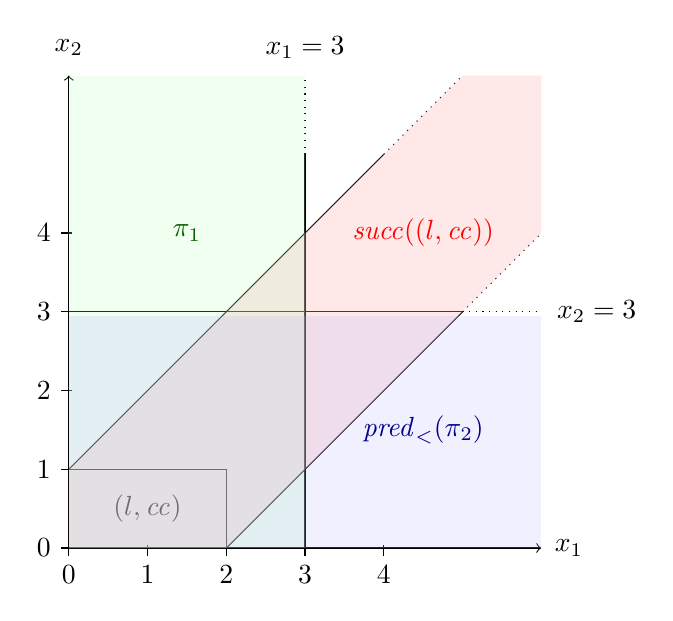
\begin{tikzpicture}
% axis
\draw[->] (0,0) -- (6, 0) coordinate (x axis);
\draw[->] (0, 0) -- (0, 6) coordinate (y axis);
% ticks
\foreach \x in {0,...,4,}
  \draw (\x,1pt) -- (\x,-3pt) node[anchor=north] {\x};
\foreach \y in {0,...,4}
  \draw (1pt,\y) -- (-3pt,\y) node[anchor=east] {\y}; 

% labels
\node[xshift=10pt] at (x axis) {$x_1$};
\node[yshift=10pt] at (y axis) {$x_2$};

% (l, cc)
\draw (0,0) rectangle (2,1);
\node at (1,0.5) {$(\loc, \region)$};

% (x_1 = 3)
\draw (3,0) -- (3,5);
\draw[dotted] (3,5) -- (3,6) coordinate (x1 label);
\node[yshift=10pt] at (x1 label) {$x_1 = 3$};

% (x_2 = 3)
\draw (0,3) -- (5,3);
\draw[dotted] (5,3) -- (6,3) coordinate (x2 label);
\node[xshift=20pt] at (x2 label) {$x_2 = 3$};

% succ((l,cc)) boundaries
\draw (0,1) -- (4,5)
      (2,0) -- (5,3);
\draw[dotted] (4,5) -- (5,6)
              (5,3) -- (6,4); 
% succ((l,cc)) shading
\draw[fill=red!30, fill opacity=0.3,draw=none] (0,0) -- (0,1) -- (5,6) -- (6,6) -- (6,4) -- (2,0);
\node[color=red] at (4.5,4) {$\suc((\loc, \region))$};

% placeholder 1
\draw[fill=green!30, fill opacity=0.2, draw=none] (0,0) rectangle (3,6);
\node[color=DarkGreen] at (1.5,4) {$\placeholder[1]$};

% pred_{<}(placeholder 2)
\draw[fill=blue!30, fill opacity=0.2, draw=none]
(0,0) rectangle (6,2.95);
\node[color=DarkBlue] at (4.5,1.5) {$\pre_{<}(\placeholder[2])$};

\end{tikzpicture}
\end{center}
In particular, the condition is not satisfied due to the triangle in which $\suc((\loc, \region))$ and $\pre_{<}(\placeholder[2])$ overlap, which is not included in $\placeholder[1]$.
To eliminate this, we must compute $\placeholder \subseteq \placeholder[2]$, such
that $\suc((\loc, \region)) \cap \pre_{<}(\placeholder)$ does not include this
\emph{bad} triangle.
%
This bad region can be identified by
\begin{equation}
\mathit{bad} \equiv (\suc((\loc, \region)) \cap \pre_{<}(\placeholder[2])) \setminus \placeholder[1].
\end{equation}
Note that $\mathit{bad}$ now contains all states in
$\suc((\loc, \region)) \cap \pre_{<}(\placeholder[2])$ that are
not in $\placeholder[1]$. In particular, we have that\todo{prove?}
\begin{equation}
\suc((\loc, \region)) \cap \pre_{<}(\placeholder[2]) \cap \overline{\suc((\loc, \region)) \cap \placeholder[1]} \subseteq \mathit{bad}
\end{equation}

The bad subset of $\placeholder[2]$ that can be reached from $\mathit{bad}$
can be computed from this as $\suc_{>}(\mathit{bad}$.

\begin{center}
  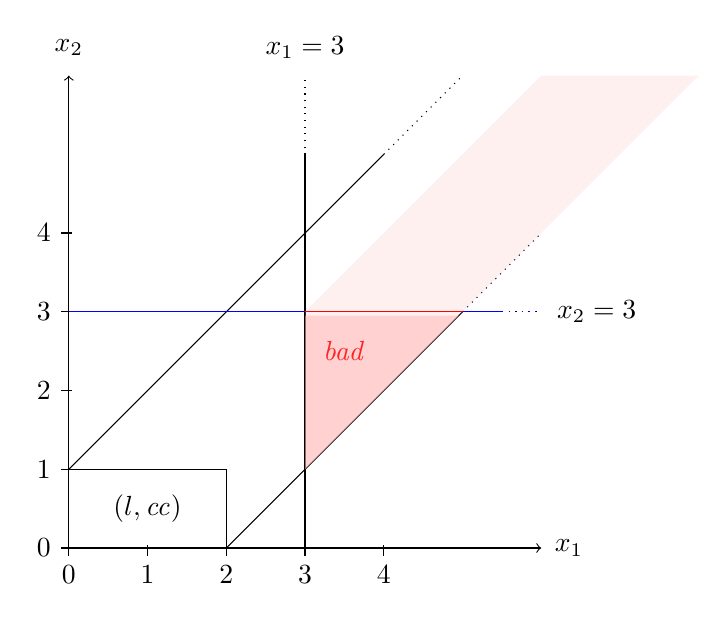
\begin{tikzpicture}
  % axis
  \draw[->] (0,0) -- (6, 0) coordinate (x axis);
  \draw[->] (0, 0) -- (0, 6) coordinate (y axis);
  % ticks
  \foreach \x in {0,...,4,}
    \draw (\x,1pt) -- (\x,-3pt) node[anchor=north] {\x};
  \foreach \y in {0,...,4}
    \draw (1pt,\y) -- (-3pt,\y) node[anchor=east] {\y}; 
  
  % labels
  \node[xshift=10pt] at (x axis) {$x_1$};
  \node[yshift=10pt] at (y axis) {$x_2$};
  
  % (l, cc)
  \draw (0,0) rectangle (2,1);
  \node at (1,0.5) {$(\loc, \region)$};
  
  % (x_1 = 3)
  \draw (3,0) -- (3,5);
  \draw[dotted] (3,5) -- (3,6) coordinate (x1 label);
  \node[yshift=10pt] at (x1 label) {$x_1 = 3$};
  
  % (x_2 = 3)
  %\draw (0,3) -- (5,3);
  \draw[dotted] (5,3) -- (6,3) coordinate (x2 label);
  \node[xshift=20pt] at (x2 label) {$x_2 = 3$};
  
  % succ((l,cc)) boundaries
  \draw (0,1) -- (4,5)
        (2,0) -- (5,3);
  \draw[dotted] (4,5) -- (5,6)
                (5,3) -- (6,4); 
  % succ((l,cc)) shading
  %\draw[fill=red!30, fill opacity=0.3,draw=none] (0,0) -- (0,1) -- (5,6) -- (6,6) -- (6,4) -- (2,0);
  %\node[color=red] at (4.5,4) {$\suc((\loc, \region))$};
  
  % placeholder 1
  %\draw[fill=green!30, fill opacity=0.2, draw=none] (0,0) rectangle (3,6);
  %\node[color=DarkGreen] at (1.5,4) {$\placeholder[1]$};
  
  % pred_{<}(placeholder 2)
  %\draw[fill=blue!30, fill opacity=0.2, draw=none]
  %(0,0) rectangle (6,2.95);
  %\node[color=DarkBlue] at (4.5,1.5) {$\pre_{<}(\placeholder[2])$};
  
  % bad
  \draw[fill=red!30,draw=none,fill opacity=0.5] (3,1) -- (3,2.95) -- (4.95,2.95) -- (3,1);
  \node[color=red] at (3.5,2.5) {$\mathit{bad}$};
  %\draw[fill=red!30,draw=none, fill opacity=0.5] (0,0) -- (1,1) -- (2,1) -- (2,0) -- (0,0);
  %\draw[fill=red!30,draw=none, fill opacity=0.2] (0,0) -- (3,2.95) -- (4.95,2.95) -- (2,0) -- (0,0);
  \draw[fill=red!30,draw=none, fill opacity=0.2] (3,3) -- (6,6) -- (8,6) -- (3,1) -- (3,3);
  
  \draw[color=red] (3,3) -- (5,3);
  \draw[color=blue] (0,3) -- (3,3);
  \draw[color=blue] (5,3) -- (5.5,3);
  \draw[color=blue, dotted] (5.5,3) -- (6,3); 

  \end{tikzpicture}
  \end{center}

To compute $\placeholder$ we need to remove those states from $\placeholder[2]$ that can be reached from $\mathit{bad}$, which is
\begin{equation}
  \placeholder \equiv \placeholder[2] \setminus \suc_{>}(\mathit{bad}).
\end{equation}
The bad part of $\placeholder[2]$
is indicated in red; the good part is indicated in blue in de the figure above.

The newly established placeholder is now such that it satisfies the side
condition, i.e., $\suc((\loc, \region)) \cap \pre_<(\placeholder) \subseteq \suc((\loc, \region)) \cap \placeholder[1]$.

% which can be achieved by
% intersecting the aforementioned region with $\placholder[1]$. The resulting value
% of $\placeholder$ is thus $\placeholder \equiv (\placeholder[2] \setminus \suc((\loc, \region) \cap \pre(\mathit{bad})) \cap \placeholder[1]$.
The resulting placeholder $\placeholder$ is indicated in the
following figure as a subset of $x_2 = 3$.

In the proof rule for relativized $\exists$, the value of $\placeholder[\exists]$
can be chosen such that $\placeholder[\exists] \equiv \pre(\placeholder)$. The
side condition $(\loc, \region) \cap \placeholder[\exists] \subseteq \pre(\placeholder)$
is then satisfied immediately. The shaded area in the following diagram gives
$\placeholder[\exists]$, $(\loc, \region) \cap \placeholder[\exists]$ is indicated
in a darker shade.

\begin{center}
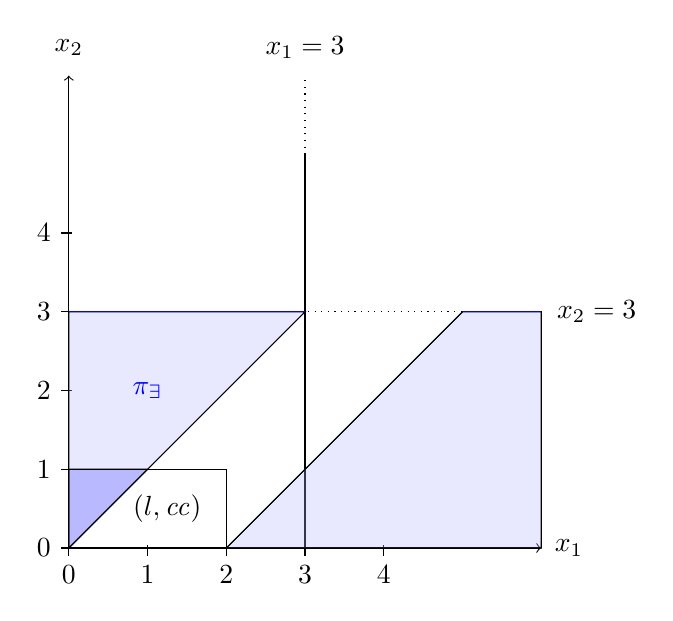
\begin{tikzpicture}
% axis
\draw[->] (0,0) -- (6, 0) coordinate (x axis);
\draw[->] (0, 0) -- (0, 6) coordinate (y axis);
% ticks
\foreach \x in {0,...,4,}
  \draw (\x,1pt) -- (\x,-3pt) node[anchor=north] {\x};
\foreach \y in {0,...,4}
  \draw (1pt,\y) -- (-3pt,\y) node[anchor=east] {\y}; 

% labels
\node[xshift=10pt] at (x axis) {$x_1$};
\node[yshift=10pt] at (y axis) {$x_2$};

% (l, cc)
\draw (0,0) rectangle (2,1);
\node at (1.25,0.5) {$(\loc, \region)$};

% (x_1 = 3)
\draw (3,0) -- (3,5);
\draw[dotted] (3,5) -- (3,6) coordinate (x1 label);
\node[yshift=10pt] at (x1 label) {$x_1 = 3$};

% (x_2 = 3)
% \draw (0,3) -- (5,3);
\draw[dotted] (0,3) -- (6,3) coordinate (x2 label);
\node[xshift=20pt] at (x2 label) {$x_2 = 3$};

% % succ((l,cc)) boundaries
\draw (2,0) -- (5,3);
% \draw[dotted] (4,5) -- (5,6)
%               (5,3) -- (6,4); 
% % succ((l,cc)) shading
% \draw[fill=red!30, fill opacity=0.3,draw=none] (0,0) -- (0,1) -- (5,6) -- (6,6) -- (6,4) -- (2,0);
% \node[color=red] at (4.5,4) {$\suc((\loc, \region))$};

% resulting placeholder
\draw[fill=blue!30, fill opacity=0.3] (0,0) -- (0,3) -- (3,3) -- (0,0);
\draw[fill=blue!30, fill opacity=0.3] (2,0) -- (5,3) -- (6,3) -- (6,0) -- (2,0);
\draw[fill=blue!70, fill opacity=0.3] (0,0) -- (0,1) -- (1,1) -- (0,0);
\node[color=blue] at (1,2) {$\placeholder[\exists]$};
\draw[color=blue] (0,3) -- (3,3);
\draw[color=blue] (5,3) -- (6,3);

% % succ((l,cc) \cap placeholder) boundaries
% \draw (0,1) -- (4,5)
%       (0,0) -- (4,4);ı
% \draw[dotted] (4,5) -- (5,6)
%                (4,4) -- (6,6); 
% % succ((l,cc) \cap \placeholder) shading
% \draw[fill=red!30, fill opacity=0.3,draw=none] (0,0) -- (0,1) -- (5,6) -- (6,6) -- (0,0);
% \node[color=red,rotate=45] at (3.5,4) {$\suc((\loc, \region) \cap \placeholder[\exists])$};

% % placeholder 1
% \draw[fill=green!30, fill opacity=0.2, draw=none] (0,0) rectangle (3,6);
% \node[color=DarkGreen] at (1.5,4) {$\placeholder[1]$};

% pred_{<}(placeholdeır 2)
% \draw[fill=blue!30, fill opacity=0.2, draw=none]
% (0,0) rectangle (6,2.95);
% \node[color=DarkBlue] at (4.5,1.5) {$\pre_{<}(\placeholder[2])$};

\end{tikzpicture}
\end{center}

\paragraph{A non-convex example}
Next, we consider an example in which the placeholder for the second subformula
of relativized exists is not convex. Consider the property 
 $\exists_{x_1 \leq 3}(x_2 = 2 \lor x_2 = 3)$, such that
 $\placeholder[1] \equiv x_1 \leq 3$, and $\placeholder[2] \equiv x_2 = 2 \lor 
 x_2 = 3$, and in which the clock region
 $(\loc, \region) \equiv 0 \leq x_1 \leq 2 \land 0 \leq x_2 \leq 1$.
 For the sake of conciseness let us write $\placeholder[2]^{1} \equiv x_2 = 2$ and
 $\placeholder[2]^2 \equiv x_2 = 3$.

First, observe that choosing $\placeholder \equiv \placeholder[2]$
does not satisfy the side condition since $\pre_{<}(x_2 = 2 \lor x _2 = 3) = x_2 < 3$, which includes states outside $x_1 \leq 3$. We show this in the following picture,
where the relevant regions are shaded ($\placeholder[1]$ green, 
$\pre_{<}(\placeholder[2])$ blue, and $\suc((\loc, \region))$ red);
$(\loc, \region)$ is the small rectangle at the bottom-left of the picture.
Note that non-convexity in this case causes the strict predecessor to be identical
to the strict predecessor of $x_2 = 3$.

\begin{center}
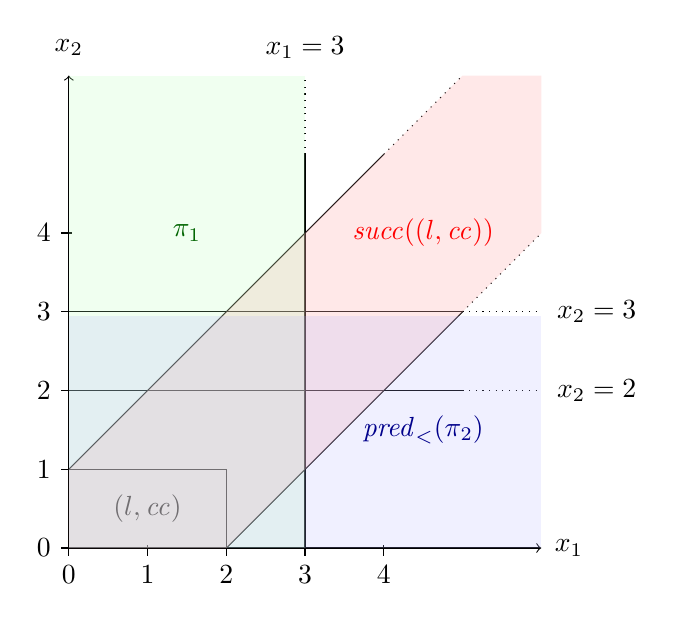
\begin{tikzpicture}
% axis
\draw[->] (0,0) -- (6, 0) coordinate (x axis);
\draw[->] (0, 0) -- (0, 6) coordinate (y axis);
% ticks
\foreach \x in {0,...,4,}
  \draw (\x,1pt) -- (\x,-3pt) node[anchor=north] {\x};
\foreach \y in {0,...,4}
  \draw (1pt,\y) -- (-3pt,\y) node[anchor=east] {\y}; 

% labels
\node[xshift=10pt] at (x axis) {$x_1$};
\node[yshift=10pt] at (y axis) {$x_2$};

% (l, cc)
\draw (0,0) rectangle (2,1);
\node at (1,0.5) {$(\loc, \region)$};

% (x_1 = 3)
\draw (3,0) -- (3,5);
\draw[dotted] (3,5) -- (3,6) coordinate (x1 label);
\node[yshift=10pt] at (x1 label) {$x_1 = 3$};

% (x_2 = 2)
\draw (0,2) -- (5,2);
\draw[dotted] (5,2) -- (6,2) coordinate (x2 label);
\node[xshift=20pt] at (x2 label) {$x_2 = 2$};

% (x_2 = 3)
\draw (0,3) -- (5,3);
\draw[dotted] (5,3) -- (6,3) coordinate (x2 label);
\node[xshift=20pt] at (x2 label) {$x_2 = 3$};

% succ((l,cc)) boundaries
\draw (0,1) -- (4,5)
      (2,0) -- (5,3);
\draw[dotted] (4,5) -- (5,6)
              (5,3) -- (6,4); 
% succ((l,cc)) shading
\draw[fill=red!30, fill opacity=0.3,draw=none] (0,0) -- (0,1) -- (5,6) -- (6,6) -- (6,4) -- (2,0);
\node[color=red] at (4.5,4) {$\suc((\loc, \region))$};

% placeholder 1
\draw[fill=green!30, fill opacity=0.2, draw=none] (0,0) rectangle (3,6);
\node[color=DarkGreen] at (1.5,4) {$\placeholder[1]$};

% pred_{<}(placeholder 2)
\draw[fill=blue!30, fill opacity=0.2, draw=none]
(0,0) rectangle (6,2.95);
\node[color=DarkBlue] at (4.5,1.5) {$\pre_{<}(\placeholder[2])$};

\end{tikzpicture}
\end{center}
In particular, the condition is not satisfied due to the triangle in which
$\suc((\loc, \region))$ and $\pre_{<}(\placeholder[2]^1)$ overlap, which is not included
in $\placeholder[1]$. To eliminate this, we must compute $\placeholder \subseteq \placeholder[2]$ such that $\suc((\loc, \region)) \cap \pre_{<}(\placeholder)$ does not include this
\emph{bad} triangle.

Now, observe that, contrary to our previous example, we cannot identify this
bad region by choosing $\mathit{bad} \equiv \suc((\loc, \region) \cap
\pre_{<}(\placeholder[2])) \setminus \placeholder[1]$ (this would lead us to
identify the same bad region as in the previous example). This is due to the
placeholder not being convex. This can be overcome by treating the convex
parts of the placeholder separately. For the good part of the placeholder w.r.t.
$\placeholder[2]^2$ we refer to the exposition given previously. We here focus
on $\placeholder[2]^1 \equiv x_2 = 2$.

With respect to $x_2 = 2$, we can identify the bad region by choosing
\begin{equation}
  \mathit{bad}^1 \equiv \suc((\loc, \region) \cap
\pre_{<}(\placeholder[2]^1)) \setminus \placeholder[1].
\end{equation} 
From this bad region we determine the bad portion op $\placeholder[2]$ as $\suc_{>}(\mathit{bad}^1)$.

\begin{center}
  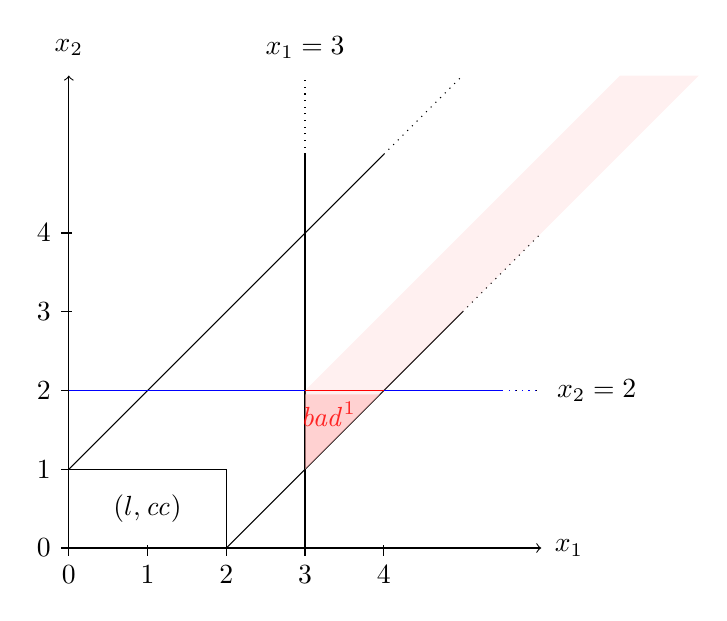
\begin{tikzpicture}
  % axis
  \draw[->] (0,0) -- (6, 0) coordinate (x axis);
  \draw[->] (0, 0) -- (0, 6) coordinate (y axis);
  % ticks
  \foreach \x in {0,...,4,}
    \draw (\x,1pt) -- (\x,-3pt) node[anchor=north] {\x};
  \foreach \y in {0,...,4}
    \draw (1pt,\y) -- (-3pt,\y) node[anchor=east] {\y}; 
  
  % labels
  \node[xshift=10pt] at (x axis) {$x_1$};
  \node[yshift=10pt] at (y axis) {$x_2$};
  
  % (l, cc)
  \draw (0,0) rectangle (2,1);
  \node at (1,0.5) {$(\loc, \region)$};
  
  % (x_1 = 3)
  \draw (3,0) -- (3,5);
  \draw[dotted] (3,5) -- (3,6) coordinate (x1 label);
  \node[yshift=10pt] at (x1 label) {$x_1 = 3$};
  
  % (x_2 = 2)
  \draw (0,2) -- (5,2);
  \draw[dotted] (5,2) -- (6,2) coordinate (x2 label);
  \node[xshift=20pt] at (x2 label) {$x_2 = 2$};
  
  % succ((l,cc)) boundaries
  \draw (0,1) -- (4,5)
        (2,0) -- (5,3);
  \draw[dotted] (4,5) -- (5,6)
                (5,3) -- (6,4); 
  % succ((l,cc)) shading
  %\draw[fill=red!30, fill opacity=0.3,draw=none] (0,0) -- (0,1) -- (5,6) -- (6,6) -- (6,4) -- (2,0);
  %\node[color=red] at (4.5,4) {$\suc((\loc, \region))$};
  
  % placeholder 1
  %\draw[fill=green!30, fill opacity=0.2, draw=none] (0,0) rectangle (3,6);
  %\node[color=DarkGreen] at (1.5,4) {$\placeholder[1]$};
  
  % pred_{<}(placeholder 2)
  %\draw[fill=blue!30, fill opacity=0.2, draw=none]
  %(0,0) rectangle (6,2.95);
  %\node[color=DarkBlue] at (4.5,1.5) {$\pre_{<}(\placeholder[2])$};
  
  % bad
  \draw[fill=red!30,draw=none,fill opacity=0.5] (3,1) -- (3,1.95) -- (3.95,1.95) -- (3,1);
  \node[color=red] at (3.3,1.7) {$\mathit{bad}^1$};
  % \draw[fill=red!30,draw=none, fill opacity=0.5] (1,0) -- (2,1) -- (2,0) -- (1,0);
  % \draw[fill=red!30,draw=none, fill opacity=0.2] (1,0) -- (3,1.95) -- (3.95,1.95) -- (2,0) -- (1,0);
  \draw[fill=red!30,draw=none, fill opacity=0.2] (3,2) -- (7,6) -- (8,6) -- (3,1) -- (3,2);
  
  \draw[color=red] (3,2) -- (4,2);
  \draw[color=blue] (0,2) -- (3,2);
  \draw[color=blue] (4,2) -- (5.5,2);
  \draw[color=blue, dotted] (5.5,2) -- (6,2); 
  
  \end{tikzpicture}
  \end{center}

We need to remove those bad states from $\placeholder[2]^1$. This gets us the new placeholder
\begin{equation}
  \placeholder^1 \equiv \placeholder[2]^1 \setminus \suc_{>}(\mathit{bad}^1).
\end{equation}
The bad part of $\placeholder[2]^1$ is indicated in red; the good part, $\placeholder^1$,
is indicated in blue in de the figure above.

Finally, we have to wonder about the value of $\placeholder$. Observe that
$\pre_{<}(\placeholder[2]^1 \lor \placeholder[2]^2) \equiv \pre_{<}(\placeholder[2]^1) \lor \pre_{<}(\placeholder[2]^2)$.

Therefore, in particular, $\suc((\loc, \region)) \cap \pre_{<}(\placeholder[2]^1 \lor \placeholder[2]^2) \subseteq \suc((\loc, \region)) \cap \placeholder[1]$ if and only if
$\suc((\loc, \region)) \cap \pre_{<}(\placeholder[2]^1) \subseteq \suc((\loc, \region)) \cap \placeholder[1] \land \suc((\loc, \region)) \cap \pre_{<}(\placeholder[2]^2) \subseteq \suc((\loc, \region)) \cap \placeholder[1]$.\todo{Prove}

Again, in the proof rule for relativized $\exists$, the value of $\placeholder[\exists]$
can be chosen such that $\placeholder[\exists] \equiv \pre(\placeholder)$. The
side condition $(\loc, \region) \cap \placeholder[\exists] \subseteq \pre(\placeholder)$
is then satisfied immediately. The shaded area in the following diagram gives
$\placeholder[\exists]$, $(\loc, \region) \cap \placeholder[\exists]$ is indicated
in a darker shade.

\begin{center}
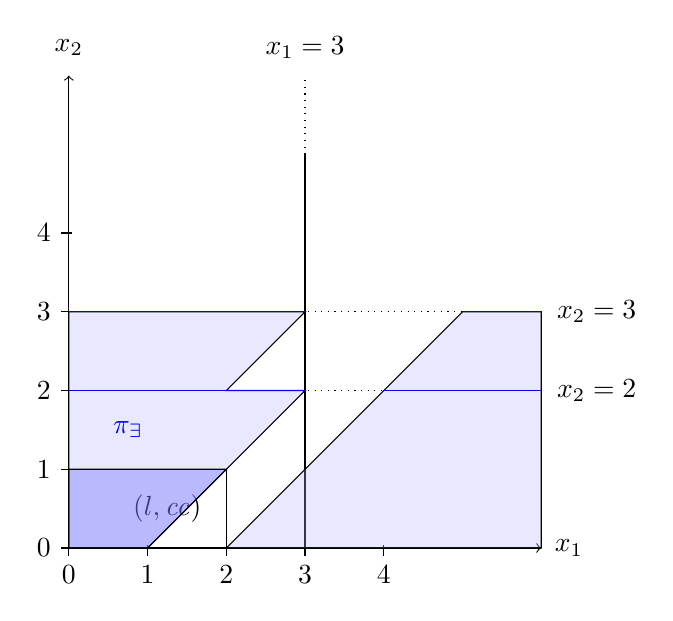
\begin{tikzpicture}
% axis
\draw[->] (0,0) -- (6, 0) coordinate (x axis);
\draw[->] (0, 0) -- (0, 6) coordinate (y axis);
% ticks
\foreach \x in {0,...,4,}
  \draw (\x,1pt) -- (\x,-3pt) node[anchor=north] {\x};
\foreach \y in {0,...,4}
  \draw (1pt,\y) -- (-3pt,\y) node[anchor=east] {\y}; 

% labels
\node[xshift=10pt] at (x axis) {$x_1$};
\node[yshift=10pt] at (y axis) {$x_2$};

% (l, cc)
\draw (0,0) rectangle (2,1);
\node at (1.25,0.5) {$(\loc, \region)$};

% (x_1 = 3)
\draw (3,0) -- (3,5);
\draw[dotted] (3,5) -- (3,6) coordinate (x1 label);
\node[yshift=10pt] at (x1 label) {$x_1 = 3$};

% (x_2 = 3)
\draw[dotted] (0,3) -- (6,3) coordinate (x2 label);
\node[xshift=20pt] at (x2 label) {$x_2 = 3$};

% (x_2 = 2)
\draw[dotted] (0,2) -- (6,2) coordinate (x2' label);
\node[xshift=20pt] at (x2' label) {$x_2 = 2$};

% % succ((l,cc)) boundaries
% \draw (0,1) -- (4,5)
%       (2,0) -- (5,3);
% \draw[dotted] (4,5) -- (5,6)
%               (5,3) -- (6,4); 
% % succ((l,cc)) shading
% \draw[fill=red!30, fill opacity=0.3,draw=none] (0,0) -- (0,1) -- (5,6) -- (6,6) -- (6,4) -- (2,0);
% \node[color=red] at (4.5,4) {$\suc((\loc, \region))$};

% resulting placeholder
\draw[fill=blue!30, fill opacity=0.3] (0,0) -- (0,3) -- (3,3) -- (2,2) -- (3,2) -- (1,0) -- (0,0);
\draw[fill=blue!30, fill opacity=0.3] (2,0) -- (5,3) -- (6,3) -- (6,0) -- (2,0);
\node[color=blue] at (.75,1.5) {$\placeholder[\exists]$};
\draw[color=blue] (0,3) -- (3,3)
                  (5,3) -- (6,3);
\draw[color=blue] (0,2) -- (3,2)
                  (4,2) -- (6,2);
\draw[fill=blue!70, fill opacity=0.3] (0,0) -- (0,1) -- (2,1) -- (1,0) -- (0,0);

% % succ((l,cc) \cap placeholder) boundaries
% \draw (0,1) -- (4,5)
%       (0,0) -- (4,4);ı
% \draw[dotted] (4,5) -- (5,6)
%                (4,4) -- (6,6); 
% % succ((l,cc) \cap \placeholder) shading
% \draw[fill=red!30, fill opacity=0.3,draw=none] (0,0) -- (0,1) -- (5,6) -- (6,6) -- (0,0);
% \node[color=red,rotate=45] at (3.5,4) {$\suc((\loc, \region) \cap \placeholder[\exists])$};

% % placeholder 1
% \draw[fill=green!30, fill opacity=0.2, draw=none] (0,0) rectangle (3,6);
% \node[color=DarkGreen] at (1.5,4) {$\placeholder[1]$};

% pred_{<}(placeholder 2)
% \draw[fill=blue!30, fill opacity=0.2, draw=none]
% (0,0) rectangle (6,2.95);
% \node[color=DarkBlue] at (4.5,1.5) {$\pre_{<}(\placeholder[2])$};

\end{tikzpicture}
\end{center}

\paragraph{An interesting, linear example (corner case)}
Next, consider a system with a single location with invariant $x < 3$, with
initial clock valuation $x = 0$. We check the property $\exists_{x < 2}(x \geq 2)$. If we use the procedure outlined above, we get the following.

First observe that $\placeholder[1] \equiv x < 2$, $\placeholder[2] \equiv x \geq 2 \land x < 3$, and $\suc((\loc, \region)) \equiv 0 \leq x < 3$.
Note that $\pre_{<}(\placeholder[2]) \equiv x < 3$. Therefore, $0 \leq x < 3 \equiv \suc((\loc, \region)) \cap \pre_{<}(\placeholder[2]) \not \subseteq \suc((\loc, \region)) \cap \placeholder[1] \equiv 0 \leq x < 2$.

According to the definition
\begin{equation}
  \mathit{bad} \equiv \suc((\loc, \region)) \cap \pre_{<}(\placeholder[2]) \cap \overline{\placeholder[1]} \equiv 0 \leq x < 3 \cap x < 3 \cap x \geq 2 \equiv 2 \leq x < 3
\end{equation}
Therefore, $\suc_{>}(\mathit{bad}) \equiv 2 < x$. The resulting placeholder we find is, therefore $\placeholder \equiv placeholder[2] \setminus \suc_{>}(\mathit{bad}) \equiv x = 2$.
Note that this placeholder satisfies the side condition.

This example also illustrates that we need to consider the strict successor of
the bad region; just taking the successor would lead to an erroneous result.

\paragraph{Pseudocode}

\begin{algorithm}[H]
  \caption{$\method{establish\_exists\_rel\_sidecondition}(\loc, \region, \placeholder[1], \placeholder[2])$}
  \begin{algorithmic}
  \IF{$\suc((\loc, \region)) \cap \pre_{<}(\placeholder[2]) \subseteq \suc((\loc, \region)) \cap \placeholder[1]$}
    \STATE $\placeholder \gets \placeholder[2]$
  \ELSE
    \STATE $\placeholder \gets \emptyset$
    \STATE Let $\placeholder[2] = \bigcup_{i=0}^{n}\placeholder[2]^i$
    \FOR{\textbf{each} $\placeholder[2]^i$ in $\placeholder[2]$}
      \STATE $\var{bad} \gets \suc((\loc, \region)) \cap \pre_{<}(\placeholder[2]^i) \cap \overline{\placeholder[1]}$
      \STATE $\placeholder^i \gets \placeholder[2]^i \cap \overline{\suc_{>}(\var{bad})}$
      \STATE $\placeholder \gets \placeholder \cup \placeholder^i$
    \ENDFOR
  \ENDIF
  \RETURN $\placeholder$
  \end{algorithmic}
\end{algorithm}

\subsection{Relativized exists, with placeholder}
If we incorporate the placeholder, we get the following proof rule.

\[
\proofrule[\exists_{r_2}]
{(\loc, \region), \placeholder[\exists] \vdash \exists_{\phi_1}(\phi_2)}
{\suc((\loc,\region)), \placeholder[2] \vdash \phi_2
\quad
\suc((\loc, \region)), \pre_{<}(\placeholder[2]) \vdash \phi_1
}
(\loc, \region) \cap \placeholder[\exists] \subseteq \pre(\placeholder[2])
\]

We again incorporate the invariant, to obtain the following.

\[
\proofrule[\exists_{r_2}]
{(\loc, \region), \placeholder[\exists] \vdash \exists_{\inv(\loc) \land \phi_1}(\inv(\loc) \land \phi_2)}
{\suc((\loc,\region)), \placeholder[2] \vdash \inv(\loc) \land \phi_2
\quad
\suc((\loc, \region)), \pre_{<}(\placeholder[2]) \vdash \inv(\loc) \land \phi_1
}
(\loc, \region) \cap \placeholder[\exists] \subseteq \pre(\placeholder[2])
\]

The derivations for the two subgoals are the same as before, only the side condition is different. We get the following proof rule.
\[
\proofrule[\exists_{r_2}]
{(\loc, \region), \placeholder[\exists] \vdash \exists_{\inv(\loc) \land \phi_1}(\inv(\loc) \land \phi_2)}
{\suc((\loc,\region)), \placeholder[2] \vdash \phi_2
\quad \suc((\loc, \region)), \placeholder[1] \vdash \phi_1
}
\begin{array}{l}
(\loc, \region) \cap \placeholder[\exists] \subseteq \pre(\placeholder[2]) \\
\placeholder[1] \subseteq \inv(\loc) \\
\placeholder[2] \subseteq \inv(\loc) \\
\suc((\loc, \region)) \cap \pre_{<}(\placeholder[2]) \subseteq \suc((\loc, \region)) \cap \placeholder[1]
\end{array}
\]

Again, as before, $\placeholder[2]$ can be too big, and we need to restrict it to $\placeholder \subseteq \placeholder[2]$ for which the sidecondition can be satisfied. We obtain the following proof rule.
\[
\proofrule
{(\loc, \region), \placeholder[\exists] \vdash \exists_{\inv(\loc) \land \phi_1}(\inv(\loc) \land \phi_2)}
{\suc((\loc,\region)), \placeholder[2] \vdash \phi_2
\quad \suc((\loc, \region)), \placeholder[1] \vdash \phi_1
}
\begin{array}{l}
(\loc, \region) \cap \placeholder[\exists] \subseteq \pre(\placeholder) \\
\placeholder[1] \subseteq \inv(\loc) \\
\placeholder[2] \subseteq \inv(\loc) \\
\placeholder \subseteq \placeholder[2] \\
\suc((\loc, \region)) \cap \pre_{<}(\placeholder) \subseteq \suc((\loc, \region)) \cap \placeholder[1]
\end{array}
\]
Note that the first side condition can easily be validated by setting $\placeholder[\exists] = \pre(\placeholder)$.

\begin{algorithm}[H]
\caption{$\method{do\_proof\_place\_exists\_rel}(\loc, \region, \placeholder[\exists], \exists_{\phi_1}(\phi_2))$}
\begin{algorithmic}
\STATE $\placeholder[2] \gets \inv(\loc)$ \COMMENT{Rule $\exists_{r_1}$}
\STATE $\method{do\_proof\_place}(\loc, \suc(\region), \placeholder[2], \phi_2)$
\IF[First subgoal fails]{$\placeholder[2] = \emptyset$}
  \STATE $\placeholder[\exists] \gets \emptyset$
\ELSE[Solve second subgoal and check side conditions]
  \STATE $\placeholder[1] \gets \infty$
  \STATE $\method{do\_proof\_place}(\loc, \suc(\region), \placeholder[1], \phi_1)$
  \IF[$\phi_2$ needs to hold immediately]{$\placeholder[1] \cap \pre_{<}(\placeholder[2]) = \emptyset$}
    \STATE $\placeholder[\exists] \gets \region \cap \placeholder[2]$
  \ELSE[Check the side conditions]
    \STATE $\placeholder \gets \method{establish\_exists\_rel\_sidecondition}(\loc, \region, \placeholder[1], \placeholder[2])$
    \STATE $\placeholder[\exists] \gets \placeholder[\exists] \cap \pre(\placeholder)$
  \ENDIF
\ENDIF
\end{algorithmic}
\end{algorithm}


\subsection{Forall}

\subsubsection{Without placeholder}

The forall rule without placeholder is described as follows.
\[
\proofrule[\forall_{t_1}]
{(\loc, \region) \vdash \forall(\phi)}
{\suc((\loc, \region)) \vdash \phi}
\]

In the implementation, care needs to be taken that only the valid time successors of $\region$ are considered,
i.e., only those time successors of $\region$ are considered that satisfy $\inv(\loc)$. To achieve this,
instead of $\forall(\phi)$, the invariant is incorporated, and the formula $\forall(\inv(\loc) \implies \phi)$
is proven. Note this formula is simplified to $\forall(\lnot \inv(\loc) \lor \phi)$.
We can now derive the following, using our rules:
\[
\proofrule[\forall_{t_1}]
{(\loc, \region) \vdash \forall(\lnot \inv(\loc) \lor \phi)}
{
\proofrule[*]{\suc((\loc, \region)) \vdash \lnot \inv(\loc) \lor \phi}
{\suc((\loc, \region)) \cap \inv(\loc) \vdash \phi
}
}
\]
where at $*$ we used the fact that $a \vdash \lnot b \lor c$ can be interpreted as
$a \implies (\lnot b \lor c)$, which is equivalent to $(a \land b) \implies c$.

The following implementation for $\forall(\phi)$ is now obtained.
\begin{algorithm}[H]
\caption{$\method{do\_proof\_forall}(\loc, \region, \forall(\phi))$}
\begin{algorithmic}
\RETURN $\method{do\_proof}(\loc, \suc(\region) \cap \inv(\loc), \phi)$
\end{algorithmic}
\end{algorithm}

\subsubsection{With placeholders}
The case of $\forall$ with placeholders is described using the following rule.
\[
\proofrule[\forall_{t_2}]
{(\loc, \region), \placeholder[\forall] \vdash \forall(\phi)}
{\suc((\loc, \region)), \placeholder \vdash \phi}
\suc((\loc, \region) \cap \placeholder[\forall]) \subseteq \suc((\loc, \region)) \land \placeholder
\]

Here we again need to incorporate the invariant, so we apply the rule
to $\forall(\lnot \inv(\loc) \lor \phi)$ instead.
\[
\proofrule[\forall_{t_2}]
{(\loc, \region), \placeholder[\forall] \vdash \forall(\lnot \inv(\loc) \lor \phi)}
{
  \proofrule[\lor_{s_2}]
  {\suc((\loc, \region)), \placeholder \vdash \lnot \inv(\loc) \lor  \phi}
  {\suc((\loc, \region)), \placeholder[1] \vdash \lnot \inv(\loc)
    \quad \suc((\loc, \region)), \placeholder[2] \vdash \phi}
    \suc((\loc, \region)) \cap \placeholder \subseteq \placeholder[1] \cup \placeholder[2]
}
\begin{array}{l}
\suc((\loc, \region) \cap \placeholder[\forall])\\
\quad \subseteq \suc((\loc, \region)) \land \placeholder
\end{array}
\]

Here we can again set $\placeholder[1] = \lnot \inv(\loc)$. If we fill this in, we get
\[
\proofrule[\forall_{t_2}]
{(\loc, \region), \placeholder[\forall] \vdash \forall(\lnot \inv(\loc) \lor \phi)}
{
  \proofrule[\lor_{s_2}]
  {\suc((\loc, \region)), \placeholder \vdash \lnot \inv(\loc) \lor  \phi}
  {\suc((\loc, \region)), \placeholder[2] \vdash \phi}
    \suc((\loc, \region)) \cap \placeholder \subseteq \lnot \inv(\loc) \cup \placeholder[2]
}
\begin{array}{l}
\suc((\loc, \region) \cap \placeholder[\forall])\\
\quad \subseteq \suc((\loc, \region)) \cap \placeholder
\end{array}
\]

When folding all this into a single rule, we get
\[
\proofrule
{(\loc, \region), \placeholder[\forall] \vdash \forall(\lnot \inv(\loc) \lor \phi)}
{\suc((\loc, \region)), \placeholder[2] \vdash \phi}
\begin{array}{l}
\suc((\loc, \region)) \cap \placeholder \subseteq \lnot \inv(\loc) \cup \placeholder[2]\\
 \suc((\loc, \region) \cap \placeholder[\forall]) \subseteq \suc((\loc, \region)) \cap \placeholder
\end{array}
\]
% Finally, observe that $\suc((\loc, \region)) \subseteq \inv(\loc)$ by definition of $\suc$, hence $\suc((\loc, \region)) \cap \placeholder \subseteq \lnot \inv(\loc) \cup \placeholder[2]$ is equivalent to saying $\suc((\loc, \region)) \cap \placeholder \subseteq \placeholder[2]$, hence the two side conditions can be collapsed into a single side condition, resulting in
% \[
% \proofrule
% {(\loc, \region), \placeholder[\forall] \vdash \forall(\lnot \inv(\loc) \lor \phi)}
% {\suc((\loc, \region)), \placeholder[2] \vdash \phi}
%  \suc((\loc, \region) \cap \placeholder[\forall]) \subseteq \placeholder[2]
% \]

The side condition is computed as follows.
\begin{algorithm}[H]
\begin{algorithmic}
  \caption{$\method{establish\_forall\_sidecondition}(\loc, \region, \placeholder[2])$}
  %\COMMENT{Establish $\placeholder[\forall]$ such that $\suc((\loc, \region) \cap \placeholder[\forall]) \subseteq \suc((\loc, \region)) \cap \placeholder$ and $\suc((\loc, \region)) \cap \placeholder \subseteq \lnot \inv(\loc) \cup \placeholder[2]$}
  \STATE $\placeholder \gets \lnot \inv(\loc) \cup \placeholder[2]$ \COMMENT{First sidecondition}
  \STATE $\mathit{\placeholder[\forall]} \gets \placeholder$
  \COMMENT{First check if $\placeholder$ is a good guess to satisfy second sidecondition}
  \IF{$\suc(\region \cap \placeholder[\forall]) \subseteq \suc(\region) \cap \placeholder$}
    \RETURN $\placeholder[\forall]$
  \ELSE
    \STATE $\mathit{bad} \gets \overline{\placeholder} \cap \suc(\region \cap \placeholder[\forall])$
    \COMMENT{Those states in $\suc(\region \cap \placeholder[\forall])$ that are outside $\placeholder$ ($\suc(\loc)$ is optimized out)}
    \STATE $\mathit{good} \gets \overline{\pre(\mathit{bad})} \cap \suc(\region)$
    \COMMENT{Essentially compute $\lnot \exists(\mathit{bad})$}
    \STATE $\placeholder[\forall] \gets \placeholder[\forall] \cap \mathit{good} \cap \suc(\loc, \region)$
    \IF[Ensure this satisfies the sidecondition]{$\suc(\region \cap \placeholder[\forall]) \subseteq \placeholder \cup \lnot \inv(\loc))$}
      \RETURN $\placeholder[\forall]$
    \ELSE[This case should not occur. To err on the side of caution, we return the empty set here]
      \RETURN $\emptyset$
    \ENDIF
  \ENDIF
\end{algorithmic}
\end{algorithm}


This gives rise to the following pseudocode.
\begin{algorithm}[H]
\caption{$\method{do\_proof\_place\_forall}(\loc, \region, \placeholder[\forall], \forall(\phi))$}
\begin{algorithmic}
\STATE $\placeholder[2] \gets \infty$
\STATE $\method{do\_proof\_place}(\loc, \suc(\region), \placeholder[2], \phi)$
\IF{$\placeholder[2] = \emptyset$}
  \STATE $\placeholder[\forall] = \emptyset$
\ELSE
  \STATE $\placeholder[\forall] \gets \method{establish\_forall\_sidecondition}(\loc, \region, \placeholder[2])$
\ENDIF
\end{algorithmic}
\end{algorithm}

\subsection{Relativized forall}

Now let us consider relativized forall. The actual proof rules are derived using~\cite[Lemma 1]{FC:14}, which states that $\forall_{\phi_1}(\phi_2) = \forall(\phi_2) \lor \exists_{\phi_2}(\phi_1 \land \phi_2)$.

Incorporating the invariant, we need to prove $\forall(\lnot \inv(\loc) \lor \phi_2) \lor \exists_{\inv(\loc) \land \phi_2}(\inv(\loc) \land \phi_1 \land \phi_2)$.

Now, let us consider the overall proof.
\[
\proofrule[\mathit{Lemma}]
{(\loc, \region) \vdash \forall_{\phi_1}(\phi_2)}
{
  \proofrule[\lor_s]
  {(\loc, \region) \vdash \forall(\lnot \inv(\loc) \lor \phi_2) \lor \exists_{\inv(\loc) \land \phi_2}(\inv(\loc) \land \phi_1 \land \phi_2)}
  {
    \proofrule[\forall_{t_2}]
    {(\loc, \region), \placeholder[\forall] \vdash \forall(\lnot \inv(\loc) \lor \phi_2)}
    {\vdots (\forall)}
    \quad
    \proofrule
    {(\loc, \region), \placeholder[\exists] \vdash \exists_{\inv(\loc) \land \phi_2}(\inv(\loc) \land \phi_1 \land \phi_2)}
    {\vdots (\exists)}
  }
  (\loc, \region) \subseteq \placeholder[\forall] \cup \placeholder[\exists]
}
\]

For the first disjunct, we simply get the analogous proof to the one for relativized forall.
\[
\proofrule
  {(\loc, \region), \placeholder[\forall] \vdash \forall(\lnot \inv(\loc) \lor \phi_2)}
  {\suc((\loc, \region)), \placeholder[2] \vdash \phi_2}
  \begin{array}{l}
    \suc((\loc, \region)) \cap \placeholder \subseteq \lnot \inv(\loc) \cup \placeholder[2]\\
    \suc((\loc, \region) \cap \placeholder[\forall]) \subseteq \suc((\loc, \region)) \cap \placeholder 
  \end{array}
\]

For the second disjunct, we derive a simplified proof using the rules for relativized exists analogous to the derivation in~\cite[Appendix C.1]{FC:14report}.

% \[
% \proofrule
% {(\loc, \region), \placeholder[\exists] \vdash \exists_{\inv(\loc) \land \phi_1}(\inv(\loc) \land \phi_2)}
% {\suc((\loc,\region)), \placeholder[2] \vdash \phi_2
% \quad \suc((\loc, \region)), \placeholder[1] \vdash \phi_1
% }
% \begin{array}{l}
% (\loc, \region) \cap \placeholder[\exists] \subseteq \pre(\placeholder) \\
% \placeholder[1] \subseteq \inv(\loc) \\
% \placeholder[2] \subseteq \inv(\loc) \\
% \placeholder \subseteq \placeholder[2] \\
% \suc((\loc, \region)) \cap \pre_{<}(\placeholder) \subseteq \suc((\loc, \region)) \cap \placeholder[1]
% \end{array}
% \]

\[
\proofrule
{(\loc, \region), \placeholder[\exists] \vdash \exists_{\inv(\loc) \land \phi_2}(\inv(\loc) \land \phi_1 \land \phi_2)}
{ \suc((\loc, \region)), \placeholder[2] \vdash \phi_2
 \quad
 {\proofrule
  {\suc((\loc, \region)), \placeholder[\land] \vdash \phi_1 \land \phi_2}
  {\vdots (\land)}}
 }
 \begin{array}{l}
  (\loc, \region) \cap \placeholder[\exists] \subseteq \pre(\placeholder') \\
  \placeholder[\land] \subseteq \inv(\loc) \\
  \placeholder[2] \subseteq \inv(\loc) \\
  \placeholder' \subseteq \placeholder[\land] \\
  \suc((\loc, \region)) \cap \pre_{<}(\placeholder') \subseteq \suc((\loc, \region)) \cap \placeholder[2]
  \end{array}
\]
Where at $\vdots (\land)$ the following subproof is performed.
\[
\proofrule[\land_p]
  {\suc((\loc, \region)), \placeholder[\land] \vdash \phi_1 \land \phi_2}
  {\suc((\loc, \region)), \placeholder[1] \vdash \phi_1
    \quad \suc((\loc, \region)), \placeholder[2] \vdash \phi_2}
  \placeholder[\land] = \placeholder[1] \cap \placeholder[2]
\]
All three subproofs share the same goal $\suc((\loc, \region)),\placeholder[2] \vdash \phi_2$. We only need to prove this subgoal once, and the rest of the work is performed in the sidecondition. Folding all this into a single proof rule we find the following proof rule.
\[
\proofrule
{(\loc, \region) \vdash \forall_{\phi_1}(\phi_2)}
{
  \suc((\loc, \region)), \placeholder[2] \vdash \phi_2
  \quad \suc((\loc, \region)), \placeholder[1] \vdash \phi_1
}
\begin{array}{l}
  (\loc, \region) \subseteq \placeholder[\forall] \cup \placeholder[\exists] \\
  \suc((\loc, \region)) \cap \placeholder \subseteq \lnot \inv(\loc) \cup \placeholder[2]\\
  \suc((\loc, \region) \cap \placeholder[\forall]) \subseteq \suc((\loc, \region)) \cap \placeholder \\
  (\loc, \region) \cap \placeholder[\exists] \subseteq \pre(\placeholder') \\
  \placeholder[\land] = \placeholder[1] \cap \placeholder[2] \\
  \placeholder[\land] \subseteq \inv(\loc) \\
  \placeholder[2] \subseteq \inv(\loc) \\
  \placeholder' \subseteq \placeholder[\land] \\
  \suc((\loc, \region)) \cap \pre_{<}(\placeholder') \subseteq \suc((\loc, \region)) \cap \placeholder[2]
\end{array}
\]

Finally, observe that we can replace the side condition $\placeholder[\land] \subseteq \inv(\loc)$ by condition $\placeholder[1] \subseteq \inv(\loc)$. The final rule is
\[
\proofrule
{(\loc, \region) \vdash \forall_{\phi_1}(\phi_2)}
{
  \suc((\loc, \region)), \placeholder[2] \vdash \phi_2
  \quad \suc((\loc, \region)), \placeholder[1] \vdash \phi_1
}
\begin{array}{l}
  (\loc, \region) \subseteq \placeholder[\forall] \cup \placeholder[\exists] \\
  \suc((\loc, \region)) \cap \placeholder \subseteq \lnot \inv(\loc) \cup \placeholder[2]\\
  \suc((\loc, \region) \cap \placeholder[\forall]) \subseteq \suc((\loc, \region)) \cap \placeholder \\
  (\loc, \region) \cap \placeholder[\exists] \subseteq \pre(\placeholder') \\
  \placeholder[1] \subseteq \inv(\loc) \\
  \placeholder[2] \subseteq \inv(\loc) \\
  \placeholder[\land] = \placeholder[1] \cap \placeholder[2] \\
  \placeholder' \subseteq \placeholder[\land] \\
  \suc((\loc, \region)) \cap \pre_{<}(\placeholder') \subseteq \suc((\loc, \region)) \cap \placeholder[2]
\end{array}
\]


\paragraph{Special cases}
Note there are some special cases here that can be used to simplify the proof. First of all, observe that if $\placeholder[1] = \emptyset$, it suffices to check
$(\loc, \region) \vdash \forall(\phi_2)$, and there is no need to involve a placeholder computation. This is consistent with ~\cite[proof rule $\forall_{ro_1}$]{FC:14report}. We immediately incorporate the invariant.

Also, if $(\loc, \region) \subseteq \placeholder[1]$ and $(\loc, \region) \subseteq \placeholder[2]$, the formula $\exists_{\phi_1}(\phi_1 \land \phi_2)$ is satisfied immediately, and $(\loc, \region) \subseteq \placeholder[\exists]$, and the other side conditions need not be checked. This corresponds to~\cite[proof rule $\forall_{ro_2}$]{FC:14}.

\[
\proofrule[\forall_{ro_1}]
{(\loc, \region) \vdash \forall_{\phi_1}(\phi_2)}
{ \proofrule[\forall_{t_1}]
  {(\loc, \region) \vdash \forall(\lnot \inv(\loc) \lor \phi_2)}
  {\suc((\loc, \region)) \cap \inv(\loc) \vdash \phi_2}
}
\quad
\proofrule[\forall_{ro_2}]
{(\loc, \region) \vdash \forall_{\phi_1}(\phi_2)}
{(\loc, \region) \vdash \phi_1 \land \phi_2}
\]
The latter rule is implemented by first checking whether $(\loc, \region) \subseteq \placeholder[1]$. Note that when this is true and $(\loc, \region) \not \subseteq \placeholder[2]$, the original property does not hold.

\begin{algorithm}[H]
\caption{$\method{do\_proof\_forall\_rel}(\loc, \region, \forall_{\phi_1}(\phi_2))$}
\begin{algorithmic}
\STATE $\placeholder[1] \gets \inv(\loc)$
\STATE $\method{do\_proof\_place}(\loc, \suc(\region), \placeholder[1], \phi_1)$
\IF[Rules $\forall_{rop_1}$ and $\forall_{t_1}$ combined]{$\placeholder[1] = \emptyset$}
  \STATE $\var{result} \gets \method{do\_proof}(\loc, \suc(\region) \cap \inv(\loc), \phi_2)$
\ELSIF[Rule $\forall_{ro_2}$]{$\region \subseteq \placeholder[1]$}
  \STATE $\var{result} \gets \method{do\_proof}(\loc, \region, \phi_2)$
\ELSE
\STATE $\placeholder[2] \gets \inv(\loc)$
\STATE $\method{do\_proof\_place}(\loc, \suc(\region), \placeholder[2], \phi_2)$
  \IF{$\placeholder[2] = \emptyset$}
    \STATE $\var{result} \gets \false$
  \ELSIF{$\suc(\region) \subseteq \placeholder[2]$}
    \STATE $\var{result} \gets \true$
  \ELSE
    \STATE $\placeholder[\forall] \gets \method{establish\_forall\_place\_sidecondition}(\loc, \region, \placeholder[2])$
    \STATE $\placeholder[\exists] \gets \method{establish\_exists\_rel\_sidecondition}(\loc, \region, \placeholder[2], \placeholder[1] \cap \placeholder[2])$
    \IF{$\placeholder[\exists] \neq \emptyset$}
      \STATE $\placeholder[\exists] \gets \pre(\placeholder[\exists] \cap \placeholder[1])$
    \ENDIF
    \STATE $\var{result} \gets \region \subseteq \placeholder[\exists] \cup \placeholder[\forall]$
  \ENDIF
\ENDIF
\RETURN $\var{result}$
\end{algorithmic}
\end{algorithm}

\subsubsection{With placeholders}
Given the use of placeholders in the derivation of the proof without placeholder, the proof rule we derived immediately extends to the case with placeholders as follows (we only add placeholder $\placeholder$, update the first sidecondition, and rename the original $\placeholder$ to $\placeholder''$).

\[
\proofrule
{(\loc, \region), \placeholder \vdash \forall_{\phi_1}(\phi_2)}
{
  \suc((\loc, \region)), \placeholder[2] \vdash \phi_2
  \quad \suc((\loc, \region)), \placeholder[1] \vdash \phi_1
}
\begin{array}{l}
  (\loc, \region) \cap \placeholder \subseteq \placeholder[\forall] \cup \placeholder[\exists] \\
  \suc((\loc, \region)) \cap \placeholder'' \subseteq \lnot \inv(\loc) \cup \placeholder[2]\\
  \suc((\loc, \region) \cap \placeholder[\forall]) \subseteq \suc((\loc, \region)) \cap \placeholder'' \\
  (\loc, \region) \cap \placeholder[\exists] \subseteq \pre(\placeholder') \\
  \placeholder[1] \subseteq \inv(\loc) \\
  \placeholder[2] \subseteq \inv(\loc) \\
  \placeholder[\land] = \placeholder[1] \cap \placeholder[2] \\
  \placeholder' \subseteq \placeholder[\land] \\
  \suc((\loc, \region)) \cap \pre_{<}(\placeholder') \subseteq \suc((\loc, \region)) \cap \placeholder[2]
\end{array}
\]

Again, there are two special cases, that extend from the previous special cases.

\[
\proofrule[\forall_{rop_1}]
{(\loc, \region), \placeholder \vdash \forall_{\phi_1}(\phi_2)}
{(\loc, \region), \placeholder \vdash \forall(\lnot \inv(\loc) \lor \phi_2)}
%
\quad
%
\proofrule[\forall_{rop_2}]
{(\loc, \region), \placeholder \vdash \forall_{\phi_1}(\phi_2)}
{(\loc, \region), \placeholder \vdash \phi_1 \land \phi_2}
\]



\begin{algorithm}[H]
  \caption{$\method{do\_proof\_place\_forall\_rel}(\loc, \region, \placeholder, \forall_{\phi_1}(\phi_2))$}
  \begin{algorithmic}
  \STATE $\placeholder[1] \gets \inv(\loc)$
  \STATE $\method{do\_proof\_place}(\loc, \suc(\region), \placeholder[1], \phi_1)$
  \IF[Essentially, the forall proof with placeholder]{$\placeholder[1] = \emptyset$}
    \STATE $\placeholder[2] \gets \placeholder$
    \STATE $\method{do\_proof\_place}(\loc, \suc(\region) \cap \inv(\loc),\placeholder[2], \phi_2)$
    \IF{$\placeholder[2] = \emptyset$}
      \STATE $\placeholder \gets \emptyset$
    \ELSE
      \STATE $\placeholder \gets \method{establish\_forall\_place\_sidecondition}(\loc, \region, \placeholder[2])$
    \ENDIF
  \ELSIF{$\placeholder[1] = \infty$}
    \STATE $\method{do\_proof\_place}(\loc, \region, \placeholder, \phi_2)$
    \COMMENT{In this case, since $\placeholder[1]$ covers everything, we are proving $\exists_{\phi_2}(\phi_2)$, which is equivalent to $\phi_2$}
  \ELSE
    \STATE $\placeholder[2] \gets \inv(\loc)$
    \STATE $\method{do\_proof\_place}(\loc, \suc(\region), \placeholder[2], \phi_2)$
    \IF{$\placeholder[2] = \emptyset$}
      \STATE $\placeholder \gets \false$
    \ELSIF[$\forall(\phi_2)$ holds, perform simple computation]{$\suc(\region) \subseteq \placeholder[2]$}
      \STATE $\placeholder \gets \placeholder[2]$
    \ELSE
      \STATE $\placeholder[\forall] \gets \method{establish\_forall\_place\_sidecondition}(\loc, \region, \placeholder[2])$
      \STATE $\placeholder[\exists] \gets \method{establish\_exists\_rel\_sidecondition}(\loc, \region, \placeholder[2], \placeholder[1] \cap \placeholder[2])$
      \IF{$\placeholder[\exists] \neq \emptyset$}
        \STATE $\placeholder[\exists] \gets \pre(\placeholder[\exists]$
      \ENDIF
      \STATE $\placeholder \gets \region \subseteq \placeholder[\exists] \cup \placeholder[\forall]$
    \ENDIF
  \ENDIF
  \end{algorithmic}
  \end{algorithm}
  

\section{Assignments}

\subsection{Clock reset}

\subsubsection{Without placeholder}
The first proof rule for clock resets performs the reset without placeholder.
\[
\proofrule[{[]}]
{(\loc, \region) \vdash \phi[\lambda := 0]}
{(\loc, \post(\region, \lambda := 0)) \vdash \phi}
\]
Now, note that, whenever $c$ is a constant, $\post(\region, \lambda := c)) = \region[\lambda := c]$. We therefore get the following proofrule.
\[
  \proofrule[{[]}]
  {(\loc, \region) \vdash \phi[\lambda := 0]}
  {(\loc, \region[\lambda := 0]) \vdash \phi}
\]
%
This results in the following pseudocode.
\begin{algorithm}[H]
  \caption{$\method{do\_proof\_reset}(\loc, \region, \phi[\lambda := 0]$}
  \begin{algorithmic}
  \RETURN $\method{do\_proof}(\loc, \region[\lambda := 0], \phi)$
  \end{algorithmic}
  \end{algorithm}

\subsubsection{With placeholder}

The authors give the following rule in~\cite{FC:14report}.
\[
\proofrule[{[]_p}]
{(\loc, \region), \placeholder[{[]}] \vdash \phi[\lambda := 0]}
{(\loc, \post(\region, \lambda := 0)), \placeholder \vdash \phi}
\placeholder[{[]}] \subseteq \placeholder[][\lambda := 0]
\]
We instead derive the rule from first principles:
\[
\proofrule
{(\loc, \region), \placeholder[{[]}] \vdash \phi[\lambda := 0]}
{(\loc, \post(\region, \lambda := 0)), \post(\placeholder[{[]}], \lambda := 0)\vdash \phi}
\]
Where we can introduce a new placeholder, and establish the corresponding sidecondition.
\[
\proofrule
{(\loc, \region), \placeholder[{[]}] \vdash \phi[\lambda := 0]}
{(\loc, \post(\region, \lambda := 0)), \placeholder \vdash \phi}
\post(\placeholder[{[]}], \lambda := 0) \subseteq \placeholder
\]
This sidecondition is equivalent to $\placeholder[{[]}] \subseteq \mathit{pre}(\placeholder, \lambda := 0)$ (property of weakest precondition and strongest postcondition). We can establish this by setting  $\placeholder[{[]}]$ to $\mathit{pre}(\placeholder, \lambda := 0)$.

Here we use the same observations as before to obtain the following proof rule.
\[
\proofrule
{(\loc, \region), \placeholder[{[]}] \vdash \phi[\lambda := 0]}
{(\loc, \region[\lambda := 0]), \placeholder \vdash \phi}
\placeholder[{[]}] \subseteq \mathit{pre}(\placeholder, \lambda := 0)
\]

\begin{algorithm}[H]
  \caption{$\method{do\_proof\_place\_reset}(\loc, \region, \placeholder, \phi[\lambda := 0]$}
  \begin{algorithmic}
    \STATE $\placeholder[1] \gets \infty$
    \STATE $\method{do\_proof\_place}(\loc, \region[\lambda := 0], \placeholder[1], \phi)$
    \STATE $\placeholder \gets \placeholder[1] \cap \mathit{pre}(\placeholder, \lambda := 0)$
  \end{algorithmic}
  \end{algorithm}

\subsection{State update}
Analogous to clock resets we have updates of the discrete state, $\phi[p := c]$, where we set control variable $p$ to value $c$.

\subsubsection{Without placeholders}
With this goes the proof rule
\[
\proofrule
{(\loc, \region) \vdash \phi[p := c]}
{(\post(\loc, p := c), \region) \vdash \phi}
\]
which simply reduces to
\[
\proofrule
{(\loc, \region) \vdash \phi[p := c]}
{(\loc[p := c], \region) \vdash \phi}
\]

\begin{algorithm}[H]
  \caption{$\method{do\_proof\_sublist}(\loc, \region, \phi[p := c]$}
  \begin{algorithmic}
  \RETURN $\method{do\_proof}(\loc[p := c], \region, \phi)$
  \end{algorithmic}
  \end{algorithm}

\subsubsection{With placeholders}
With this goes the proof rule
\[
\proofrule
{(\loc, \region), \placeholder \vdash \phi[p := c]}
{(\post(\loc, p := c), \region), \placeholder \vdash \phi}
\]
which simply reduces to
\[
\proofrule
{(\loc, \region), \placeholder \vdash \phi[p := c]}
{(\loc[p := c], \region), \placeholder \vdash \phi}
\]

\begin{algorithm}[H]
  \caption{$\method{do\_proof\_place\_sublist}(\loc, \region, \placeholder, \phi[p := c]$}
  \begin{algorithmic}
  \STATE $\method{do\_proof\_place}(\loc[p := c], \region, \placeholder, \phi)$
  \end{algorithmic}
  \end{algorithm}


\subsection{Clock assignment}

Copying one clock to another, i.e., $\phi[x := y]$ for $x,y$ clocks, is similar to clock reset.

\subsubsection{Without placeholder}
We have the following rule (not listed in \cite{FC:14report}).
\[
\proofrule
{(\loc, \region) \vdash \phi[x := y]}
{(\loc, \post(\region, x := y)) \vdash \phi}
\]
Analogous to what we saw before, $ \post(\region, x := y) = \region[x := y]$, so we get the following proofrule.
\[
  \proofrule[{[]}]
  {(\loc, \region) \vdash \phi[x := y]}
  {(\loc, \region[x := y]) \vdash \phi}
\]
%
This results in the following pseudocode.
\begin{algorithm}[H]
  \caption{$\method{do\_proof\_assign}(\loc, \region, \phi[x := y]$}
  \begin{algorithmic}
  \RETURN $\method{do\_proof}(\loc, \region[x := y], \phi)$
  \end{algorithmic}
  \end{algorithm}

\subsubsection{With placeholder}
This is, again, analogous to the clock reset.
\[
\proofrule
{(\loc, \region), \placeholder[{[]}] \vdash \phi[x := y]}
{(\loc, \post(\region, x := y)), \post(\placeholder[{[]}], x := y)\vdash \phi}
\]
Where we can introduce a new placeholder, and establish the corresponding sidecondition.
\[
\proofrule
{(\loc, \region), \placeholder[{[]}] \vdash \phi[x := y]}
{(\loc, \post(\region, x := y)), \placeholder \vdash \phi}
\post(\placeholder[{[]}], x := y) \subseteq \placeholder
\]
This sidecondition is equivalent to $\placeholder[{[]}] \subseteq \mathit{pre}(\placeholder, x := y)$ (property of weakest precondition and strongest postcondition). We can establish this by setting  $\placeholder[{[]}]$ to $\mathit{pre}(\placeholder, x := y)$.

Here we use the same observations as before to obtain the following proof rule.
\[
\proofrule
{(\loc, \region), \placeholder[{[]}] \vdash \phi[x := y]}
{(\loc, \post(\region, x := y)), \placeholder \vdash \phi}
\placeholder[{[]}] \subseteq \mathit{pre}(\placeholder, x := y)
\]

\begin{algorithm}[H]
  \caption{$\method{do\_proof\_place\_assign}(\loc, \region, \placeholder, \phi[x := y]$}
  \begin{algorithmic}
    \STATE $\placeholder[1] \gets \infty$
    \STATE $\method{do\_proof\_place}(\loc, \region[x := y], \placeholder[1], \phi)$
    \STATE $\placeholder \gets \placeholder \cap \mathit{pre}(\placeholder[1], x := y)$
  \end{algorithmic}
  \end{algorithm}

\subsection{State assignment}
Analogous to clock assignments there is a state assignment $
\phi[p := q]$ where discrete state variable $p$ is assigned the value of $q$. 


\subsubsection{Without placeholders}
With this goes the proof rule
\[
\proofrule
{(\loc, \region) \vdash \phi[p := q]}
{(\post(\loc, p := q), \region) \vdash \phi}
\]
which simply reduces to
\[
\proofrule
{(\loc, \region) \vdash \phi[p := q]}
{(\loc[p := q], \region) \vdash \phi}
\]

\begin{algorithm}[H]
  \caption{$\method{do\_proof\_sublist}(\loc, \region, \phi[p := q]$}
  \begin{algorithmic}
  \RETURN $\method{do\_proof}(\loc[p := q], \region, \phi)$
  \end{algorithmic}
  \end{algorithm}

\subsubsection{With placeholders}
With this goes the proof rule
\[
\proofrule
{(\loc, \region), \placeholder \vdash \phi[p := q]}
{(\post(\loc, p := q), \region), \placeholder \vdash \phi}
\]
which simply reduces to
\[
\proofrule
{(\loc, \region), \placeholder \vdash \phi[p := q]}
{(\loc[p := q], \region), \placeholder \vdash \phi}
\]

\begin{algorithm}[H]
  \caption{$\method{do\_proof\_place\_sublist}(\loc, \region, \placeholder, \phi[p := q]$}
  \begin{algorithmic}
  \STATE $\method{do\_proof\_place}(\loc[p := q], \region, \placeholder, \phi)$
  \end{algorithmic}
  \end{algorithm}



\section{Modalities}

\subsection{Box modality}

\subsubsection{Without placeholders}

Note that the implementation does not only support clock resets, but also clock assignments of the form $x := y$, where $x$ and $y$ are clocks. In the code below we therefore write $(\loc, a, g, \lambda, \sigma, \loc')$ for transitions, instead of just $(\loc, a, g, \lambda, \loc')$. Here $\lambda$ contains the clocks that are reset, and $\sigma$ contains assignments $x_1 := y_1, \ldots x_n := y_n$.
We base ourselves on the proof rule for singular hybrid automata by Cleaveland and Keiren.
\[
\proofrule
{(\loc, \region) \vdash [a] \phi}
{(\loc_1, (\region \land g_1)[\lambda_1 := 0][\vec{x}_1 := \vec{y}_1] \land \inv(\loc_1) \vdash \phi
\quad
\cdots
\quad
(\loc_n, (\region \land g_n)[\lambda_n := 0][\vec{x}_n := \vec{y}_n] \land \inv(\loc_n) \vdash \phi
}
\]
where$ \{(\loc,a,g_i,\lambda_i,\loc_i) \mid 1 \leq i \leq n \} = \{ (l', a', g, \lambda, l'') \in E \mid l = l' \land a = a' \}$

Fontana and Cleaveland \cite{FC:14report} given the following alternative for timed automata.
\[
\proofrule[{[a]_{\mathit{Act}}}]
{(\loc, \region) \vdash [a]\phi}
{(\loc_1, \region \land g_1) \vdash \phi{[\lambda_1 := 0][\vec{x}_1 := \vec{y}_1]}
\quad \cdots \quad
(\loc_n, \region \land g_n) \vdash \phi{[\lambda_n := 0][\vec{x}_n := \vec{y}_n]}
}
\]
where $\bigcup_i \{ (g_i,\lambda_i,\loc_i) \} = \{ (\loc', g', \lambda') \mid (\loc, a, g', \lambda', \loc') \in E \}$.

This rule ignores the invariant of the target location, so should be modified to read:
\[
\proofrule[{[a]_{\mathit{Act}}}]
{(\loc, \region) \vdash [a]\phi}
{
\begin{array}{c}
  (\loc_1, \region \land g_1) \vdash (\inv(\loc_1) \implies \phi){[\lambda_1 := 0][\vec{x}_1 := \vec{y}_1]} \\
 \cdots \\
(\loc_n, \region \land g_n) \vdash (\inv(\loc_n) \implies \phi){[\lambda_n := 0][\vec{x}_n := \vec{y}_n]}
\end{array}
}
\]
where $\bigcup_i \{ (g_i,\lambda_i,\loc_i) \} = \{ (\loc', g', \lambda') \mid (\loc, a, g', \lambda', \loc') \in E \}$. 
Note that we can carry the weakest precondition over to the left hand side, and obtain:
\[
\proofrule[{[a]_{\mathit{Act}}}]
{(\loc, \region) \vdash [a]\phi}
{
\begin{array}{c}
 (\loc_1, \region \land g_1 \land \inv(\loc_1)[\lambda_1 := 0][\vec{x}_1 := \vec{y}_1]) \vdash \phi{[\lambda_1 := 0][\vec{x}_1 := \vec{y}_1]} \\
\cdots \\
(\loc_n, \region \land g_n \land \inv(\loc_n)[\lambda_n := 0][\vec{x}_n := \vec{y}_n]) \vdash \phi{[\lambda_n := 0][\vec{x}_n := \vec{y}_n]}
\end{array}
}
\]
where $\bigcup_i \{ (g_i,\lambda_i,\loc_i) \} = \{ (\loc', g', \lambda') \mid (\loc, a, g', \lambda', \loc') \in E \}$.

For timed automata, the rules are equivalent. This can be seen from the following derivation.
\begin{align*}
  & \post(\region \land g, \lambda := 0, \vec{x} := \vec{y}) \land \inv(\loc') \subseteq \phi \\
\iff & \post(\region \land g, \lambda := 0, \vec{x} := \vec{y}) \subseteq \inv(\loc') \implies \phi \\
\iff & \post(\region \land g, \lambda := 0, \vec{x} := \vec{y}) \subseteq \lnot \inv(\loc') \lor \phi \\
\iff & \region \land g \subseteq \wpre(\lnot \inv(\loc') \lor \phi, \lambda := 0, \vec{x} := \vec{y})\\
\iff & \region \land g \subseteq \wpre(\lnot \inv(\loc'), \lambda := 0, \vec{x} := \vec{y}) \lor \wpre(\phi, \lambda := 0, \vec{x} := \vec{y})\\
\iff & \region \land g \subseteq \lor \wpre(\phi, \lambda := 0, \vec{x} := \vec{y})\\
\iff & \region \land g \land \wpre(\inv(\loc'), \lambda := 0, \vec{x} := \vec{y}) \subseteq \wpre(\phi, \lambda := 0, \vec{x} := \vec{y}) \\
\iff & \region \land g \land \wpre(\inv(\loc'), \lambda := 0, \vec{x} := \vec{y}) \subseteq \phi[\lambda := 0][\vec{x} := \vec{y}]
\end{align*}
where $\post(\region \land g, \lambda := 0, \vec{x} := \vec{y})$ is a shorthand for $\post(\post(\region \land g, \lambda := 0), \vec{x} := \vec{y})$, and likewise for $\wpre$.

Note that the proof rule can trivially be generalised to cover all actions.
\[
\proofrule[{[-]_{\mathit{Act}}}]
{(\loc, \region) \vdash [-]\phi}
{(\loc, \region) \vdash [a_1]\phi
\quad \cdots \quad
(\loc, \region) \vdash [a_n]\phi}
\Sigma = \{ a_1, \ldots, a_n \}
\]

Using the version of the proof rule from~\cite{FC:14report}, we obtain the following pseudocode.
\begin{algorithm}[H]
  \caption{$\method{do\_proof\_allact}(\loc, \region, [-]\phi$}
  \begin{algorithmic}
  \STATE $\var{result} \gets \mathit{true}$
  \FOR{$(\loc, a, g, \lambda, \loc') \in E$}
    \IF{$\region \cap g \neq \emptyset$}
      \IF{$\inv(\loc') \neq \emptyset$}
        \STATE $\var{inv} \gets \mathit{pre}(\inv(\loc'), \lambda := 0)$
        \FOR{$x_i := y_1 \text{ in } \sigma$}
          \STATE $\var{inv} \gets \mathit{pre}(\var{inv}, x_i := y_i)$
        \ENDFOR
        \IF{$\region \cap g \cap \var{inv} \neq \emptyset$}
          \STATE $\var{result} \gets \method{do\_proof}(\loc, \region \cap g \cap \var{inv}, \phi)$
        \ENDIF
      \ENDIF
    \ENDIF
  \ENDFOR
  \end{algorithmic}
  \end{algorithm}

\subsubsection{With placeholders}
The version of the proof rule with placeholders is more involved. Note that no rule for this case is given in~\cite{FC:14report}.

We can, however, easily derive an algorithm from the proof rule without placeholders as follows.
\[
\proofrule
{(\loc, \region), \placeholder \vdash [a] \phi}
{
\begin{array}{c}
(\loc_1, (\region \land \placeholder \land g_1)[\lambda_1 := 0][\vec{x}_1 := \vec{y}_1] \land \inv(\loc_1) \vdash \phi\\
\cdots\\
(\loc_n, (\region \land \placeholder \land g_n)[\lambda_n := 0][\vec{x}_n := \vec{y}_n] \land \inv(\loc_n) \vdash \phi
\end{array}
}
\]
The subgoal, for an arbitrary $i$, here corresponds with
\[
  \post(\region \land \placeholder \land g_i, \lambda_i := 0, \vec{x}_i := \vec{y}_i) \land \inv(\loc_i) \subseteq \phi
  \]
Using the derivation shown before, we find this is equivalent to 
\[
  \region \land \placeholder \land g_i \land \wpre(\inv(\loc_i), \lambda_i := 0, \vec{x}_i := \vec{y}_i) \subseteq \wpre(\phi,\lambda_i := 0, \vec{x}_i := \vec{y}_i)
\]
Then we find for $\placeholder$, that
\[
  \placeholder \subseteq \lnot(\region \land g_i) \lor \lnot \wpre(\inv(\loc_i), \lambda_i := 0, \vec{x}_i := \vec{y}_i) \lor \wpre(\phi,\lambda_i := 0, \vec{x}_i := \vec{y}_i)
\]

For the sake of completeness, we write the proof rule with individual placeholders for each subgoal:
\[
\proofrule
{(\loc, \region), \placeholder \vdash [a] \phi}
{\begin{array}{c}
(\loc_1, (\region \land \placeholder[1] \land g_1)[\lambda_1 := 0][\vec{x}_1 := \vec{y}_1] \land \inv(\loc_1) \vdash \phi \\
\cdots \\
(\loc_n, (\region \land \placeholder[n] \land g_n)[\lambda_n := 0][\vec{x}_n := \vec{y}_n] \land \inv(\loc_n) \vdash \phi
\end{array}
}
\placeholder \implies \bigwedge_{i=1}^n \placeholder[n]
\]
where $\bigcup_i \{ (g_i,\lambda_i,\loc_i) \} = \{ (\loc', g', \lambda') \mid (\loc, a, g', \lambda', \loc') \in E \}$.

Also, the alternative in the style of Fontana and Cleaveland is the following.
\[
\proofrule[{[a]_{\mathit{Act}}}]
{(\loc, \region) \vdash [a]\phi}
{
\begin{array}{c}
 (\loc_1, \region \land g_1 \land \inv(\loc_1)[\lambda_1 := 0][\vec{x}_1 := \vec{y}_1]), \placeholder[1] \vdash \phi{[\lambda_1 := 0][\vec{x}_1 := \vec{y}_1]} \\
\cdots \\
(\loc_n, \region \land g_n \land \inv(\loc_n)[\lambda_n := 0][\vec{x}_n := \vec{y}_n]), \placeholder[n] \vdash \phi{[\lambda_n := 0][\vec{x}_n := \vec{y}_n]}
\end{array}
}
\placeholder \implies \bigwedge_{i=1}^n \placeholder[i]
\]
where $\bigcup_i \{ (g_i,\lambda_i,\loc_i) \} = \{ (\loc', g', \lambda') \mid (\loc, a, g', \lambda', \loc') \in E \}$.

Using this idea, the algorithm becomes the following.

\begin{algorithm}[H]
  \caption{$\method{do\_proof\_place\_allact}(\loc, \region, \placeholder, [-]\phi$}
  \begin{algorithmic}
  \FOR{$(\loc, a, g, \lambda, \loc') \in E$}
    \STATE $\region_g \gets \region \cap g$
    \STATE $\placeholder[g] \gets \placeholder \cap g$    
    \IF{$\region_g \neq \emptyset \land \placeholder[g] \neq \emptyset$}
      \STATE $\var{inv} \gets \inv(\loc')$
      \IF{$\inv(\loc') \neq \emptyset$}
        \STATE $\var{inv} \gets \mathit{pre}(\var{inv}, \lambda := 0)$
        \FOR{$x_i := y_1 \text{ in } \sigma$}
          \STATE $\var{inv} \gets \mathit{pre}(\var{inv}, x_i := y_i)$
        \ENDFOR
      \ENDIF
      \STATE $\method{do\_proof\_place}(\loc, \region_g \cap \var{inv}, \placeholder[e] \cap \var{inv}, \phi)$
      \STATE $\placeholder \gets \placeholder \cap (\placeholder[e] \cup \lnot \var{inv} \cup \lnot \placeholder[g])$
    \ENDIF
  \ENDFOR
  \end{algorithmic}
  \end{algorithm}


\subsection{Diamond modality}

\subsubsection{Without placeholder}
For the diamond modality, the proof rules listed in~\cite{FC:14report} are incomplete. We here formulate a rule which is a generalisation of $\lor_s$, and a variation of the rule for $[a]$.

\[
\proofrule
{(\loc, \region) \vdash \langle a \rangle \phi}
{
\begin{array}{c}
(\loc_1, (\region \land \placeholder[1] \land g_1)[\lambda_1 := 0][\vec{x}_1 := \vec{y}_1] \land \inv(\loc_1) \vdash \phi \\
\cdots \\
(\loc_n, (\region \land \placeholder[n] \land g_n)[\lambda_n := 0][\vec{x}_n := \vec{y}_n] \land \inv(\loc_n) \vdash \phi
\end{array}
}
\region \implies \bigvee_{i=1}^n (\region \land g_i \land \placeholder[i])
\]
where $\bigcup_i \{ (g_i,\lambda_i,\loc_i) \} = \{ (\loc', g', \lambda') \mid (\loc, a, g', \lambda', \loc') \in E \}$.

We can again give the rule in the style of Fontana and Cleaveland as follows.
\[
\proofrule[{\langle a \rangle_{\mathit{Act}}}]
{(\loc, \region) \vdash \langle a \rangle \phi}
{
\begin{array}{c}
 (\loc_1, \region \land g_1 \land \inv(\loc_1)[\lambda_1 := 0][\vec{x}_1 := \vec{y}_1]), \placeholder[1] \vdash \phi{[\lambda_1 := 0][\vec{x}_1 := \vec{y}_1]} \\
\cdots \\
(\loc_n, \region \land g_n \land \inv(\loc_n)[\lambda_n := 0][\vec{x}_n := \vec{y}_n]), \placeholder[n] \vdash \phi{[\lambda_n := 0][\vec{x}_n := \vec{y}_n]}
\end{array}
}
\region \implies \bigvee_{i=1}^n (\region \land g_i \land \placeholder[i])
\]
where $\bigcup_i \{ (g_i,\lambda_i,\loc_i) \} = \{ (\loc', g', \lambda') \mid (\loc, a, g', \lambda', \loc') \in E \}$.

This generalises to $\langle - \rangle$ in the obvious way.

We get the following pseudocode.
\begin{algorithm}[H]
  \caption{$\method{do\_proof\_existact}(\loc, \region, \langle - \rangle \phi$}
  \begin{algorithmic}
  \STATE $\placeholder[\langle \rangle] \gets \emptyset$
  \FOR{$(\loc, a, g, \lambda, \loc') \in E$}
    \STATE $\region_g \gets \region \cap g$
    \STATE $\placeholder[g] \gets g$    
    \IF[Check this is the correct guard]{$\region_g \neq \emptyset \land \placeholder[g] \neq \emptyset$}
      \STATE $\var{inv} \gets \inv(\loc')$
      \IF{$\inv(\loc') \neq \emptyset$}
        \STATE $\var{inv} \gets \mathit{pre}(\var{inv}, \lambda := 0)$
        \FOR{$x_i := y_1 \text{ in } \sigma$}
          \STATE $\var{inv} \gets \mathit{pre}(\var{inv}, x_i := y_i)$
        \ENDFOR
      \ENDIF
      \STATE $\placeholder[g] \gets \placeholder[g] \cap \var{inv}$
      \STATE $\method{do\_proof\_place}(\loc, \region_g \cap \var{inv}, \placeholder[g], \phi)$
      \STATE $\placeholder[\langle \rangle] \gets \placeholder[\langle \rangle] \cup \placeholder[g]$
    \ENDIF
  \ENDFOR
  \RETURN $\region \subseteq \placeholder[\langle \rangle]$
  \end{algorithmic}
  \end{algorithm}

\subsubsection{With placeholder}
\[
\proofrule
{(\loc, \region), \placeholder \vdash \langle a \rangle \phi}
{
\begin{array}{c}
(\loc_1, (\region \land \placeholder[1] \land g_1)[\lambda_1 := 0][\vec{x}_1 := \vec{y}_1] \land \inv(\loc_1) \vdash \phi \\
\cdots \\
(\loc_n, (\region \land \placeholder[n] \land g_n)[\lambda_n := 0][\vec{x}_n := \vec{y}_n] \land \inv(\loc_n) \vdash \phi
\end{array}
}
\region \land \placeholder \implies \bigvee_{i=1}^n (\region \land g_i \land \placeholder[i])
\]
where $\bigcup_i \{ (g_i,\lambda_i,\loc_i) \} = \{ (\loc', g', \lambda') \mid (\loc, a, g', \lambda', \loc') \in E \}$.

Again, in the alternative style from Fontana and Cleaveland, we get the following rule.
\[
\proofrule[{\langle a \rangle_{\mathit{Act}}}]
{(\loc, \region), \placeholder \vdash \langle a \rangle \phi}
{
\begin{array}{c}
 (\loc_1, \region \land g_1 \land \inv(\loc_1)[\lambda_1 := 0][\vec{x}_1 := \vec{y}_1]), \placeholder[1] \vdash \phi{[\lambda_1 := 0][\vec{x}_1 := \vec{y}_1]} \\
\cdots \\
(\loc_n, \region \land g_n \land \inv(\loc_n)[\lambda_n := 0][\vec{x}_n := \vec{y}_n]), \placeholder[n] \vdash \phi{[\lambda_n := 0][\vec{x}_n := \vec{y}_n]}
\end{array}
}
\region \land \placeholder \implies \bigvee_{i=1}^n (\region \land g_i \land \placeholder[i])
\]
where $\bigcup_i \{ (g_i,\lambda_i,\loc_i) \} = \{ (\loc', g', \lambda') \mid (\loc, a, g', \lambda', \loc') \in E \}$.

\begin{algorithm}[H]
  \caption{$\method{do\_proof\_place\_existact}(\loc, \region, \placeholder, \langle - \rangle \phi$}
  \begin{algorithmic}
  \STATE $\placeholder[\langle \rangle] \gets \emptyset$
  \FOR{$(\loc, a, g, \lambda, \loc') \in E$}
    \STATE $\region_g \gets \region \cap g$
    \STATE $\placeholder[g] \gets \placeholder \cap g$    
    \IF[Check this is the correct guard]{$\region_g \neq \emptyset \land \placeholder[g] \neq \emptyset$}
      \STATE $\var{inv} \gets \inv(\loc')$
      \IF{$\inv(\loc') \neq \emptyset$}
        \STATE $\var{inv} \gets \mathit{pre}(\var{inv}, \lambda := 0)$
        \FOR{$x_i := y_1 \text{ in } \sigma$}
          \STATE $\var{inv} \gets \mathit{pre}(\var{inv}, x_i := y_i)$
        \ENDFOR
      \ENDIF
      \STATE $\placeholder[g] \gets \placeholder[g] \cap \var{inv}$
      \STATE $\method{do\_proof\_place}(\loc, \region_g \cap \var{inv}, \placeholder[g], \phi)$
      \STATE $\placeholder[\langle \rangle] \gets \placeholder[\langle \rangle] \cup \placeholder[g]$
    \ENDIF
  \ENDFOR
  \STATE $\placeholder \gets \placeholder \cap \placeholder[\langle \rangle]$
  \end{algorithmic}
  \end{algorithm}

\subsection{Ablewaitinf}

$\exists(z . (\forall (z \leq 1)))$

\subsection{Unablewaitinf}

$\forall(z . (\exists (z \leq 1)))$


\bibliographystyle{alpha}
\bibliography{hybrid}

\end{document}